\documentclass[11pt,a4paper]{article}
\usepackage[margin=2.3cm]{geometry}
\usepackage{amsmath,amssymb}
\usepackage{booktabs,longtable,array}
\usepackage{graphicx}
\usepackage{float}
\usepackage{xcolor}
\usepackage{enumitem}
\usepackage{microtype}
\usepackage{fancyhdr}
\usepackage[hidelinks]{hyperref}
\usepackage{caption}
\usepackage{tikz}
\definecolor{ink}{HTML}{12263A}
\definecolor{accent}{HTML}{1F6FB5}
\graphicspath{{../results/}}
\setlength{\parindent}{0pt}
\setlength{\parskip}{0.55em}
\renewcommand{\arraystretch}{1.18}
\setlist{itemsep=0.15em,topsep=0.2em}
\pagestyle{fancy}
\fancyhf{}
\fancyhead[L]{\small Battery Module Studio}
\fancyhead[R]{\small Formulas and calculations}
\fancyfoot[C]{\small\thepage}
\renewcommand{\headrulewidth}{0.3pt}
\captionsetup{font=small,labelfont=bf}
\newcommand{\ds}[1]{\textsc{DS}~#1}
\newcommand{\degC}{\ensuremath{{}^{\circ}\mathrm{C}}}
\newcommand{\Rbus}{R_{\mathrm{bus}}}
\newcommand{\nS}{n_{\mathrm{S}}}
\newcommand{\nP}{n_{\mathrm{P}}}

\begin{document}

\begin{center}
{\LARGE\bfseries\color{ink} Battery Module Studio}\\[0.4em]
{\Large\color{accent} Formulas, calculations and graph definitions}\\[0.6em]
{\small TELIPORT Season 4: Reusable Digital Platform for Designing Battery Energy System\\
Cell: LG INR21700-M50 \quad|\quad Simulation only \quad|\quad 31 October 2026}
\end{center}

\vspace{0.4em}
\hrule
\vspace{0.6em}

\textbf{How to use this document.} Every number the dashboard shows is produced by a formula written here, in the order the code evaluates it. Each section names the source file. Parameter sources are tagged: \emph{DS} is the LG Chem product specification INR21700 M50 18.20Wh (2016-08-23, status ``Tentative''), with section number; \emph{BD} is the batterydesign.net page ``LG INR 21700 M50'' (5 May 2023), mainly its DCIR-versus-temperature chart; \emph{PB} is the PyBaMM \texttt{Chen2020} parameter set (Chen et al., J.~Electrochem.~Soc.~167, 080534, 2020); \emph{FIT} is a value fitted offline to PB; \emph{assumption} is in none of these, and the reason is given. Numbers in the worked examples use the default settings: 4S3P module, 35\,\degC\ ambient, 1C discharge, 0.6C charge, two back-to-back cycles, 5\,\% resistance spread, seed 7.

\textbf{What the sources do not contain.} The M50 specification is a tentative draft. It has no open-circuit-voltage curve, no capacity-versus-rate table, no charge-time data and no thermal data. The platform therefore takes its OCV curve and its diffusion behaviour from PB, its resistance temperature dependence from a chart in BD, and says in Section~\ref{sec:val} which validation rows are independent checks and which only reproduce an input.

\tableofcontents

%--------------------------------------------------------------------
\section{Model structure}
%--------------------------------------------------------------------
The module has $\nS$ series groups, each with $\nP$ cells in parallel, so $N=\nS\nP$ cells. The default is $\nS=4$, $\nP=3$, $N=12$. Cell $k=(g-1)\nP+i$ sits in series group $g=1,\dots,\nS$ at parallel position $i=1,\dots,\nP$. On the physical grid, series groups are columns and parallel positions are rows.

Five subsystems share one parameter set (\texttt{Design}, \texttt{Scenario}, \texttt{Requirements}):
\begin{enumerate}
\item \textbf{Electrical}: open-circuit voltage, a series resistance and one polarisation branch per cell, current sharing, charge and discharge limits (Section~\ref{sec:elec}).
\item \textbf{Heat}: ohmic and polarisation losses per cell and in the interconnects (Section~\ref{sec:heat}).
\item \textbf{Thermal}: a network of one node per cell plus an optional plate (Section~\ref{sec:therm}).
\item \textbf{BMS}: voltage cut-offs and temperature trips (Section~\ref{sec:bms}).
\item \textbf{Parts and checks}: mass, cost, volume, requirement checks and ranking (Sections~\ref{sec:parts}--\ref{sec:rank}).
\end{enumerate}
A sixth layer, \textbf{liquid cooling} for Design D (Section~\ref{sec:liquid}), adds a cold plate, coolant, radiator and pump to the same thermal network. A seventh, \textbf{electrochemical} (Section~\ref{sec:echem}), adds a lithium-plating screen taken from the PyBaMM Chen2020 model. It reads a stored table, so the platform runs without PyBaMM.

%--------------------------------------------------------------------
\section{Notation}
%--------------------------------------------------------------------
\begin{longtable}{@{}p{2.3cm}p{8.4cm}p{3.6cm}@{}}
\toprule
Symbol & Meaning & Unit or default \\
\midrule
\endhead
$\nS,\ \nP,\ N$ & series groups, parallel cells per group, cell count & 4, 3, 12 \\
$Q$ & cell capacity, defines 1C & 4.85\,Ah (\ds{2.1}, \ds{2.9}) \\
$s$ & state of charge (SOC), 0 to 1 & -- \\
$\mathrm{OCV}(s)$ & open-circuit voltage of one cell & V, Table~\ref{tab:ocv} \\
$R_{0}$, $R_{1}$, $\tau$ & series resistance, polarisation resistance, polarisation time constant at 25\,\degC & 24.78\,m$\Omega$, 14.07\,m$\Omega$, 65\,s \\
$C_1$ & polarisation capacitance, $C_1=\tau/R_1$ & 4.62\,kF \\
$\mu_k$ & resistance spread factor of cell $k$ & -- \\
$f(T)$ & resistance multiplier vs temperature & -- \\
$R_{0,k},R_{1,k}$ & $R_0\mu_kf(T_k)$ and $R_1\mu_kf(T_k)$ & $\Omega$ \\
$V_{1,k}$ & polarisation voltage across $R_1\parallel C_1$ of cell $k$ & V \\
$\Rbus$ & total interconnect resistance of the string & 4\,m$\Omega$ \\
$I$ & module current, positive on discharge & A \\
$I_k$ & current in cell $k$, same sign convention & A \\
$c_{\mathrm{dis}},c_{\mathrm{chg}}$ & discharge and charge rate in multiples of $Q$ & C \\
$T_k$ & temperature of node $k$ & \degC \\
$T_{\mathrm{amb}}$ & ambient temperature & 35\,\degC \\
$C_k$ & heat capacity of node $k$ & J/K \\
$G_{\mathrm{amb},k}$ & conductance from node $k$ to ambient & W/K \\
$g_{\mathrm{nb}}$ & conductance between neighbouring cells & W/K \\
$h_{\mathrm{eff}}$ & effective convection coefficient & W/m$^2$/K \\
$\Delta t$ & time step & 5\,s (10\,s in sweeps) \\
\bottomrule
\end{longtable}

%--------------------------------------------------------------------
\section{Cell data and their sources}\label{sec:cell}
%--------------------------------------------------------------------
All values are in Appendix~A with their source tags. The ones that drive the formulas are: capacity $Q=4.85$\,Ah (minimum capacity; $1\mathrm{C}=4\,850$\,mA, which is how the datasheet converts 0.3C to 1\,455\,mA, 0.7C to 3\,395\,mA and 1.5C to 7\,275\,mA), nominal voltage 3.63\,V, charge voltage $4.20\pm0.05$\,V, discharge cut-off 2.50\,V, mass 68\,g, diameter $\le21.10$\,mm, height $\le70.15$\,mm, DC resistance $30\pm6$\,m$\Omega$ (0.5C, 30\,s, 25\,\degC, 50\,\% SOC, \ds{4.3.2}), 1\,kHz impedance $\le25$\,m$\Omega$ (\ds{4.3.1}).

\begin{longtable}{@{}p{3.2cm}p{5.3cm}p{5.8cm}@{}}
\toprule
 & Charge & Discharge \\
\midrule
\endhead
Temperature window & 0 to 45\,\degC\ (\ds{5.1}) & $-20$ to 60\,\degC\ (\ds{5.1}) \\
Maximum current & 0.3C (1.455\,A) from 0 to 25\,\degC; 0.7C (3.395\,A) from 25 to 50\,\degC\ (\ds{2.6}) & 0.3C (1.455\,A) from $-20$ to 5\,\degC; 1.5C (7.275\,A) from 5 to 60\,\degC\ (\ds{2.9}) \\
End condition & 50\,mA after a standard charge (\ds{2.4}); C/20 in the cycle-life test (\ds{4.2.3}) & 2.50\,V \\
\bottomrule
\end{longtable}
\ds{2.6} lists charge current up to 50\,\degC, while \ds{5.1} limits charging to 0 to 45\,\degC. The model uses the stricter 45\,\degC. The datasheet gives no release temperature after a trip, so a 5\,K hysteresis is assumed (charge releases at 40\,\degC, discharge at 55\,\degC).

%--------------------------------------------------------------------
\section{Electrical sub-model}\label{sec:elec}
%--------------------------------------------------------------------
\emph{Source: \texttt{bms/cell.py}, \texttt{bms/sim.py}.} Each cell is $\mathrm{OCV}(s)$ in series with $R_{0,k}$ and a parallel branch $R_{1,k}\parallel C_1$ (Figure~\ref{fig:circuit}). The branch stands for solid-state diffusion in the electrodes. It lengthens the constant-voltage charge tail and lowers the energy delivered at high rate, which a resistor alone cannot do. It captures these effects only in part (Section~\ref{sec:val}).

\begin{figure}[H]
\centering
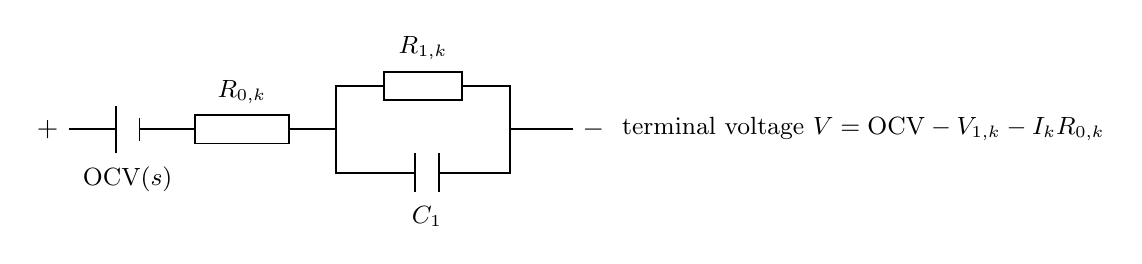
\begin{tikzpicture}[x=1cm,y=1cm,>=stealth,line width=0.7pt]
\draw (0,0) node[left]{$+$} -- (0.6,0);
\draw (0.6,-0.3) -- (0.6,0.3);
\draw (0.9,-0.15) -- (0.9,0.15);
\node[below] at (0.75,-0.35) {\small OCV$(s)$};
\draw (0.9,0) -- (1.6,0);
\draw (1.6,-0.18) rectangle (2.8,0.18); \node[above] at (2.2,0.2) {\small $R_{0,k}$};
\draw (2.8,0) -- (3.4,0);
\draw (3.4,0) -- (3.4,0.55) -- (4.0,0.55); \draw (4.0,0.37) rectangle (5.0,0.73); \node[above] at (4.5,0.75) {\small $R_{1,k}$};
\draw (5.0,0.55) -- (5.6,0.55) -- (5.6,0);
\draw (3.4,0) -- (3.4,-0.55) -- (4.4,-0.55); \draw (4.4,-0.8) -- (4.4,-0.3); \draw (4.7,-0.8) -- (4.7,-0.3); \draw (4.7,-0.55) -- (5.6,-0.55) -- (5.6,0);
\node[below] at (4.55,-0.85) {\small $C_1$};
\draw (5.6,0) -- (6.4,0) node[right]{$-$};
\node[right] at (6.9,0) {\small terminal voltage $V=\mathrm{OCV}-V_{1,k}-I_kR_{0,k}$};
\end{tikzpicture}
\caption{Equivalent circuit of one cell. $V_{1,k}$ is the voltage across the $R_1\parallel C_1$ branch.}\label{fig:circuit}
\end{figure}

\subsection{Open-circuit voltage}
$\mathrm{OCV}(s)$ is piecewise linear through the 16 points in Table~\ref{tab:ocv}. They come from PB: a C/50 discharge of the \texttt{Chen2020} single-particle model at 25\,\degC, with the voltage read at equal steps of discharged capacity ($s=1-\text{discharged fraction}$). The script \texttt{tools/make\_ocv.py} regenerates them. This is a research parameterisation of an M50 cell, not a datasheet curve. Against the datasheet it gives $E=17.8$\,Wh at 0.2C (17.6 minimum, 18.2 nominal) and a mean discharge voltage of 3.68\,V (3.63 nominal).

\begin{table}[H]
\centering
\small
\begin{tabular}{@{}l*{8}{c}@{}}
\toprule
SOC (\%) & 0 & 2 & 5 & 10 & 15 & 20 & 30 & 40 \\
OCV (V) & 2.500 & 2.859 & 3.105 & 3.292 & 3.430 & 3.481 & 3.578 & 3.663 \\
\midrule
SOC (\%) & 50 & 60 & 70 & 80 & 90 & 95 & 98 & 100 \\
OCV (V) & 3.746 & 3.836 & 3.944 & 4.037 & 4.093 & 4.118 & 4.157 & 4.196 \\
\bottomrule
\end{tabular}
\caption{Open-circuit voltage table (PB, 25\,\degC).}\label{tab:ocv}
\end{table}

\subsection{Resistance, temperature and cell spread}
The two resistances of cell $k$ are
\begin{equation}
R_{0,k}=R_{0}\,\mu_k\,f(T_k),\qquad R_{1,k}=R_{1}\,\mu_k\,f(T_k),\qquad \tau_k=R_{1,k}\,C_1 ,
\end{equation}
so the capacitance $C_1$ is constant and the time constant scales with $R_1$. The multiplier $f(T)$ is read from the BD chart of DCIR (0.5\,s pulse) against temperature, which has three clusters of points. The means are 68\,m$\Omega$ at 10\,\degC\ (points 59, 70, 76), 23\,m$\Omega$ at 25\,\degC\ (21, 23, 25) and 14.2\,m$\Omega$ at 45\,\degC\ (14, 14.5). These were read from the chart by eye, with an uncertainty of about 2\,m$\Omega$. Dividing by the 25\,\degC\ mean gives $f(10)=2.957$, $f(25)=1$, $f(45)=0.615$. Between the points $\ln f$ is interpolated linearly in $T$. Below 10\,\degC\ the 10--25\,\degC\ slope is extended, and above 45\,\degC\ the 45\,\degC\ value is held (so heat is not under-estimated when hot). Examples: $f(15)=2.060$, $f(35)=0.784$, $f(45)=0.615$, $f(60)=0.615$. Only the ratios are used; the absolute 25\,\degC\ value comes from \ds{4.3.2}.

The cell-to-cell spread is
\begin{equation}
\mu_k=\operatorname{clip}\big(1+\sigma\,\xi_k,\ 0.7,\ 1.6\big),\qquad \xi_k\sim\mathcal{N}(0,1),
\end{equation}
with $\sigma=0.05$ by default and $\xi_k$ drawn from a seeded generator (\texttt{numpy.random.default\_rng(seed)}). The same seed gives the same result every run. The spread is applied to both $R_0$ and $R_1$.

\subsection{Fitting \texorpdfstring{$R_0$, $R_1$, $\tau$}{R0, R1, tau}}
The datasheet gives only the 30\,s resistance, so the split between $R_0$ and $R_1$ and the time constant come from a fit (\texttt{tools/fit\_polarisation.py}):
\begin{enumerate}
\item In the PB DFN model at 25\,\degC, start at 50\,\% SOC, rest 10\,min, discharge at 0.5C for 20\,min, rest 30\,min.
\item Fit the circuit voltage change to the DFN voltage change by least squares over the pulse and relaxation. Result: $R_0=29.89$\,m$\Omega$, $R_1=16.98$\,m$\Omega$, $\tau=65$\,s, rms error 3.0\,mV. A second branch did not reduce the error, so one branch is used.
\item The DFN cell is more resistive than the datasheet: the fitted circuit gives a 30\,s resistance of 36.2\,m$\Omega$ (38.4\,m$\Omega$ when read from the voltage as in \ds{4.3.2}, which includes the open-circuit-voltage drop over the 30\,s) against $30\pm6$. Both $R_0$ and $R_1$ are multiplied by one factor, $30/36.2=0.829$, so that $R_0+R_1(1-e^{-30/\tau})=30$\,m$\Omega$. This gives the values used: $R_0=24.78$, $R_1=14.07$\,m$\Omega$.
\end{enumerate}
The fit uses nothing from charge or high-rate tests, so those stay independent (Section~\ref{sec:val}). After scaling, the 0.5\,s resistance is 24.9\,m$\Omega$, inside the 21 to 25\,m$\Omega$ range of the BD points at 25\,\degC, and this was not fitted.

\subsection{Polarisation state}
With $I_k$ positive on discharge, over a step $\Delta t$ the branch is integrated exactly,
\begin{equation}
V_{1,k}^{n+1}=V_{1,k}^{n}\,e^{-\Delta t/\tau_k}+I_k\,R_{1,k}\,\big(1-e^{-\Delta t/\tau_k}\big).
\end{equation}
During charge $I_k<0$, so $V_{1,k}$ is negative and adds to the terminal voltage.

\subsection{Parallel groups and current sharing}
Cells in group $g$ share one terminal voltage $V_g$. From $I_{g,i}=(\mathrm{OCV}-V_{1,g,i}-V_g)/R_{0,g,i}$ and $\sum_i I_{g,i}=I$:
\begin{equation}
S_g=\sum_{i=1}^{\nP}\frac{1}{R_{0,g,i}},\quad U_g=\sum_{i=1}^{\nP}\frac{V_{1,g,i}}{R_{0,g,i}},\quad
V_g=\underbrace{\mathrm{OCV}-\frac{U_g}{S_g}}_{A_g}-\underbrace{\frac{1}{S_g}}_{B_g}\,I .
\end{equation}
A cell with lower $R_0$, including a hotter one, carries more current. All series groups carry the same module current. The module voltage is $V_{\mathrm{mod}}=\sum_g V_g-I\Rbus$.

\subsection{Rates and state of charge}
Rates are multiples of the cell capacity:
\begin{equation}
I_{\mathrm{dis}}=c_{\mathrm{dis}}\,\nP\,Q,\qquad I_{\mathrm{chg}}=c_{\mathrm{chg}}\,\nP\,Q .
\end{equation}
At 1C with $\nP=3$: $I=1\times3\times4.85=14.55$\,A in the module and 4.85\,A in an average cell. The SOC is updated each step as
\begin{equation}
s_{n+1}=\operatorname{clip}\!\Big(s_n-\frac{I\,\Delta t}{3600\,\nP\,Q},\ 0,\ 1\Big),
\end{equation}
with $I$ negative on charge. Coulombic efficiency is taken as 1. All cells share one SOC, so capacity mismatch is not modelled.

\subsection{Discharge}
Discharge ends when any of three conditions holds:
\begin{equation}
\min_g\frac{A_g-2.50}{B_g}<I_{\mathrm{dis}},\qquad s\le0,\qquad 1-s\ \ge\ \rho(\bar T).
\end{equation}
The first is the voltage cut-off at the requested current. The third uses the energy retention table of \ds{4.4.4} (0.2C, charged at 25\,\degC): $\rho=0.70,0.80,1.00,0.95$ at $-10,0,25,60$\,\degC, interpolated linearly in the mean cell temperature $\bar T$ and held outside the table. The resistance alone gives 94\,\% at 0\,\degC\ and 86\,\% at $-10$\,\degC\ (Section~\ref{sec:val}), so the table adds what the circuit cannot explain. At 35\,\degC\ it removes about 1.4\,\%.

\subsection{Constant-current, constant-voltage charge}
The largest charge current that keeps every group at or below 4.20\,V is
\begin{equation}
I_{V}=\min_g\frac{4.20-A_g}{B_g}.
\end{equation}
The constant-current (CC) phase holds $I=I_{\mathrm{chg}}$ until $I_V\le I_{\mathrm{chg}}$. The constant-voltage (CV) phase then follows $I=\min(I_{\mathrm{chg}},\max(I_V,0))$, so the current falls as the cells fill and $V_{1}$ relaxes. Charging stops when
\begin{equation}
I\le I_{\mathrm{cut}}=\nP\,i_{\mathrm{term}},\qquad i_{\mathrm{term}}=\begin{cases}0.050\ \mathrm{A}& i_{\mathrm{chg,cell}}\le1.455\ \mathrm{A}\ (\ds{2.4})\\ Q/20=0.2425\ \mathrm{A}&\text{otherwise}\ (\ds{4.2.3})\end{cases}
\end{equation}
or when $s\ge1$. For the default 0.6C charge $I_{\mathrm{cut}}=0.73$\,A for the module. In rest phases $I=0$ and the polarisation voltage relaxes with $\tau_k$. Energy in a phase is
\begin{equation}
E=\sum_n V_{\mathrm{mod},n}\,|I_n|\,\frac{\Delta t}{3600}\quad[\mathrm{Wh}].
\end{equation}

\subsection{Current limits as a check, not a clamp}
The datasheet current limits depend on temperature (table in Section~\ref{sec:cell}). The simulation does not clamp the current to them, so the checker can show a charger that does not match the cell. For each step the ratio
\begin{equation}
\rho_I=\max_k\frac{|I_k|}{I_{\lim}\big(\operatorname{clip}(T_k,T_{\min},T_{\max})\big)}
\end{equation}
is recorded, and checks L3 and L4 report its maximum. The temperature is clipped into the window so that $\rho_I$ measures only the current-versus-band mismatch. Temperatures outside the window are reported by the temperature checks.

\textbf{Why 0.6C is the default charge rate.} The datasheet maximum is 0.7C, i.e. 3.395\,A per cell. A charger set to 0.7C splits the current between parallel cells in proportion to $1/R_0$, and with a 5\,\% spread the most conductive cell carries about 4\,\% more than the 3.395\,A, so L4 fails in every design. At 0.6C the same cell reaches 89\,\% of the limit.

%--------------------------------------------------------------------
\section{Heat generation}\label{sec:heat}
%--------------------------------------------------------------------
Each cell produces
\begin{equation}
Q_k=I_k^{2}R_{0,k}+\frac{1}{2}\,\frac{(V_{1,k}^{n})^{2}+(V_{1,k}^{n+1})^{2}}{R_{1,k}}+\frac{I^{2}\Rbus}{N},
\end{equation}
the loss in $R_0$, the loss in $R_1$ (average of the start and end of the step), and the interconnect loss spread equally over all cells. Entropic (reversible) heat is neglected because no M50 value is available in the sources (the PB set has it equal to zero). The module-level energy balance, terminal energy equal to OCV energy minus heat minus change of energy stored in $C_1$, is checked in \texttt{tests/test\_model.py}.

Example at 1C in steady state, 35\,\degC\ (default 4S3P): $R_0+R_1=30.46$\,m$\Omega$ at $f=0.784$, so $Q_{\text{cell}}=4.85^{2}\times0.03046=0.716$\,W per cell. The interconnect loss is $14.55^{2}\times0.004=0.847$\,W for the string. The module total is $12\times0.716+0.847=9.44$\,W. During the first minutes $V_1$ has not built up and the loss is lower, which is why the temperature curve starts with a gentler slope.

%--------------------------------------------------------------------
\section{Thermal network}\label{sec:therm}
%--------------------------------------------------------------------
\emph{Source: \texttt{build\_thermal} and \texttt{simulate} in \texttt{bms/sim.py}.}
There is one temperature node per cell, plus one node for the aluminium plate if the design has one.

\subsection{Heat capacity}
\begin{equation}
C_k=m_{\mathrm{cell}}\,c_p=0.068\times900=61.2\ \mathrm{J/K},\qquad
C_{\mathrm{sp}}=\rho_{\mathrm{Al}}\,A_{\mathrm{sp}}\,t_{\mathrm{sp}}\,c_{\mathrm{Al}} .
\end{equation}
The cell specific heat $c_p=900$ J/kg/K is an assumption: typical cylindrical Li-ion cells fall between 800 and 1100, and neither the specification nor the BD page gives an M50 value. The PB layer values (700 J/kg/K for electrodes and separator, 385 and 897 for the collectors) cover the jelly roll only, not the steel can. The sensitivity run varies it. For the plate, $\rho_{\mathrm{Al}}=2700$ kg/m$^3$, $c_{\mathrm{Al}}=900$ J/kg/K. With $A_{\mathrm{sp}}=125$ cm$^2$ and $t_{\mathrm{sp}}=2$ mm (design B) the plate weighs 67.5 g and $C_{\mathrm{sp}}=60.8$ J/K.

\subsection{Convection to ambient}
The effective coefficient is
\begin{equation}
h_{\mathrm{eff}}=h_{\mathrm{nat}}+\begin{cases}k_f\,v^{0.6}&v>0\\0&v=0\end{cases},\qquad h_{\mathrm{nat}}=10,\ k_f=12 .
\end{equation}
Natural convection plus radiation $h_{\mathrm{nat}}=10$ W/m$^2$/K is an assumption. The forced-air term is a bank-derated power law (assumption): a 2\,m/s fan gives $h_{\mathrm{eff}}=10+12\times2^{0.6}=28.2$ W/m$^2$/K.

Each cell has four vertical sides (north, south, east, west on the grid). The surface area of one side is
\begin{equation}
a_{\mathrm{side}}=\frac{\pi D L}{4}=\frac{\pi\times0.0211\times0.07015}{4}=11.63\ \mathrm{cm}^2 .
\end{equation}
A side facing a neighbour is only partly open to the air. Its exposure depends on the gap $s$:
\begin{equation}
\varphi(s)=1-\exp\!\left(-\frac{s}{s_0}\right),\qquad s_0=3\ \mathrm{mm}\ \text{(assumption)} .
\end{equation}
So $\varphi(1.5\ \mathrm{mm})=0.393$ and $\varphi(4\ \mathrm{mm})=0.736$. With $n_{b,k}$ the number of neighbouring cells of cell $k$ (4-connected grid), the conductance to ambient is
\begin{equation}
G_{\mathrm{amb},k}=h_{\mathrm{eff}}\,a_{\mathrm{side}}\Big[(4-n_{b,k})+\varphi(s)\,n_{b,k}\Big].
\end{equation}
Corner cells have 2 neighbours, edge cells 3, and the two interior cells of a $4\times3$ grid have 4. Cell tops and bottoms are treated as insulated.

\begin{table}[H]
\centering
\begin{tabular}{@{}lccc@{}}
\toprule
$G_{\mathrm{amb}}$ (W/K) & Corner & Edge & Interior \\
\midrule
A, B (1.5\,mm gap, natural convection) & 0.0324 & 0.0253 & 0.0183 \\
C (4\,mm gap, 2\,m/s fan) & 0.1138 & 0.1052 & 0.0965 \\
\bottomrule
\end{tabular}
\caption{Conductance from each cell to ambient. Interior cells cool worst, which creates the hotspot.}
\end{table}

\subsection{Conduction between neighbouring cells}
Through the air gap, with an effective contact width of $0.4D$ (assumption) and a minimum gap of 0.5\,mm:
\begin{equation}
g_{\mathrm{nb}}=\frac{k_{\mathrm{air}}\,L\,(0.4D)}{\max(s,0.5\ \mathrm{mm})},\qquad k_{\mathrm{air}}=0.026\ \mathrm{W/m/K}.
\end{equation}
This gives $0.0103$ W/K at 1.5\,mm and $0.0038$ W/K at 4\,mm.

\subsection{Spreader plate (design B)}
Each cell connects to the plate through a thermal pad, and the plate sheds heat from both faces:
\begin{equation}
g_{cs}=\frac{k_{\mathrm{pad}}\,A_{\mathrm{pad}}}{t_{\mathrm{pad}}}=\frac{1.5\times5\times10^{-4}}{1\times10^{-3}}=0.75\ \mathrm{W/K},\qquad
G_{\mathrm{sp,amb}}=2\,h_{\mathrm{eff}}\,A_{\mathrm{sp}}=2\times10\times0.0125=0.25\ \mathrm{W/K}.
\end{equation}
The pad conductivity 1.5 W/m/K and the pad geometry are assumptions. The plate area (125\,cm$^2$, about twice the 61\,cm$^2$ footprint of the cell block) and the pad contact patch (5\,cm$^2$ per cell) are design choices fixed before the sensitivity run; Section~\ref{sec:sens} varies the pad conductivity.

\subsection{Governing equation and solver}
Collecting all nodes into vectors,
\begin{equation}
\mathbf{C}\,\frac{d\mathbf{T}}{dt}=-\mathbf{K}\,\mathbf{T}+\mathbf{Q}+\mathbf{G}_{\mathrm{amb}}\,T_{\mathrm{amb}},\qquad
\mathbf{K}=\mathbf{L}+\operatorname{diag}(\mathbf{G}_{\mathrm{amb}}),
\end{equation}
where $\mathbf{L}$ is the weighted graph Laplacian built from $g_{\mathrm{nb}}$ and $g_{cs}$ ($L_{kk}=\sum_j g_{kj}$, $L_{kj}=-g_{kj}$). The plate node has no heat source. Backward Euler is used,
\begin{equation}
\Big(\tfrac{\mathbf{C}}{\Delta t}+\mathbf{K}\Big)\mathbf{T}^{n+1}=\tfrac{\mathbf{C}}{\Delta t}\mathbf{T}^{n}+\mathbf{Q}^{n}+\mathbf{G}_{\mathrm{amb}}T_{\mathrm{amb}} .
\end{equation}
The matrix depends only on the design, so it is inverted once per run. The scheme is stable for any step size, which matters because the plate node has a time constant of a few seconds.

\subsection{Time constants and a hand check}
For a lumped estimate, $\tau_{\mathrm{th}}=\sum C/\sum G_{\mathrm{amb}}$ and the long-time rise is $\Delta T_\infty=Q_{\mathrm{tot}}/\sum G_{\mathrm{amb}}$.
\begin{center}
\begin{tabular}{@{}lcccc@{}}
\toprule
Design & $\sum G_{\mathrm{amb}}$ (W/K) & $\tau_{\mathrm{th}}$ & $\Delta T_\infty$ at 35\,\degC\ & Simulated mean cell, end of discharge \\
\midrule
A & 0.3183 & 2307 s (38 min) & 29.7 K & 53.8\,\degC \\
B & 0.5683 & 1399 s (23 min) & 16.6 K & 47.5\,\degC \\
C & 1.2793 & 162 s (10 min) & 7.4 K & 41.4\,\degC \\
\bottomrule
\end{tabular}
\end{center}
For design A at 1C: $Q_{\mathrm{tot}}=9.44$\,W gives $\Delta T_\infty=29.7$\,K when $R$ is taken at 35\,\degC. At a cell temperature near 50\,\degC\ the resistance is lower ($f=0.615$), $Q_{\mathrm{tot}}=7.59$\,W and $\Delta T_\infty=23.8$\,K. A first-order rise after $t=58$\,min covers $1-e^{-t/\tau_{\mathrm{th}}}=0.78$ of the way, so the mean cell temperature should be about 54 to 58\,\degC. The simulated mean at the end of the discharge is 53.8\,\degC. This is a sanity check on the thermal solver, not a validation against a measurement.

%--------------------------------------------------------------------
\section{BMS and protection logic}\label{sec:bms}
%--------------------------------------------------------------------
The BMS sees the temperature of one sensor cell, $T_s$: cell 0 (a corner) for \texttt{corner}, cell $\lfloor \nS/2\rfloor\nP+\lfloor\nP/2\rfloor$ for \texttt{center}, or $\max_k T_k$ for \texttt{hottest} (ideal sensing).

\begin{center}
\begin{tabular}{@{}lccc@{}}
\toprule
Mode & Trip when & Release when & Source \\
\midrule
Discharge & $T_s\ge60$\,\degC & $T_s\le55$\,\degC & \ds{5.1}, release assumed \\
Charge & $T_s\ge45$\,\degC & $T_s\le40$\,\degC & \ds{5.1}, release assumed \\
Charge inhibit & $\min_k T_k<0$\,\degC & automatic & \ds{5.1} \\
Discharge end & $\min_g (A_g-2.5)/B_g<I_{\mathrm{dis}}$ & -- & \ds{2.7} \\
Charge CC to CV & $I_V\le I_{\mathrm{chg}}$ & -- & \ds{2.5} \\
\bottomrule
\end{tabular}
\end{center}
When tripped the current is set to zero and the time is counted as trip time. The charge cut-off acts on the sensor reading, not on the hottest cell. With the corner sensor under-reading the hotspot by several kelvin, the BMS can allow charging while the hottest cell is above 45\,\degC. Design A shows this: the sensor holds the string near 45\,\degC, and the hottest cell reaches 53.1\,\degC\ during charge (check L1). The BMS also trips only at datasheet limits, so a design can break the application requirement without the BMS reacting (check I2).

%--------------------------------------------------------------------
\section{Duty cycle and time stepping}\label{sec:cycle}
%--------------------------------------------------------------------
The run starts fully charged at ambient temperature and repeats \emph{discharge, rest, charge, rest} for \texttt{n\_cycles} cycles. Rest lasts 10\,min. Each phase is capped at 8\,h. At every step $\Delta t$:
\begin{enumerate}
\item Compute $R_{0,k}$, $R_{1,k}$, $A_g$, $B_g$ from the current temperatures and polarisation states.
\item Read the sensor temperature and update the trip state.
\item Test the phase end conditions (Sections~\ref{sec:elec} and \ref{sec:bms}). Set the module current $I$.
\item Compute cell currents $I_k$, heat $Q_k$, group voltages and $V_{\mathrm{mod}}$. Record the step, including the limit ratio $\rho_I$.
\item Add $V_{\mathrm{mod}}|I|\Delta t/3600$ to the phase energy, update $s$ and $V_{1,k}$.
\item Solve the thermal step for $\mathbf{T}^{n+1}$ and advance time.
\end{enumerate}
Results are always taken from the first discharge and first charge (cold start) for energy and charge time, and over the whole run for peak temperatures. The second cycle starts warm, which is why the peak occurs late.

%--------------------------------------------------------------------
\section{Indicators}\label{sec:ind}
%--------------------------------------------------------------------
\emph{Source: \texttt{indicators} in \texttt{bms/sim.py}.}
Let $T_{\max}(t)=\max_k T_k(t)$ and $T_{\min}(t)=\min_k T_k(t)$ over the cell nodes only (the plate node is excluded).
\begin{align*}
E_{\mathrm{use}} &= E_{\mathrm{dis},1}-P_{\mathrm{fan}}\,\frac{t_{\mathrm{dis},1}}{3600}
&&\text{usable energy, net of fan energy, first discharge}\\
T_{\mathrm{peak}} &= \max_t T_{\max}(t)
&&\text{peak cell temperature, whole run}\\
\Delta T_{\mathrm{spread}} &= \max_t\big[T_{\max}(t)-T_{\min}(t)\big]
&&\text{largest temperature difference between cells}\\
t_{\mathrm{chg}} &= \text{duration of the first charge phase}
&&\text{includes the CV tail and BMS pauses}\\
\eta_{\mathrm{rt}} &= E_{\mathrm{dis},1}/E_{\mathrm{chg},1}
&&\text{round trip, SOC returns to 100\,\%, fan excluded}\\
I_{\mathrm{cell,max}} &= \max_t \max_k |I_k(t)|
&&\text{reported separately for discharge and charge}\\
\rho_{I} &= \max_t \max_k |I_k|/I_{\lim}(T_k)
&&\text{limit ratio, discharge and charge}\\
V_{g,\min} &= \min_{t,g} V_g(t)
&&\text{lowest group voltage}\\
\delta_{\mathrm{sensor}} &= \max_t\big[T_{\max}(t)-T_s(t)\big]
&&\text{how much the sensor under-reads the hotspot}\\
\rho_E &= E_{\mathrm{use}}/m,\qquad \rho_V=E_{\mathrm{use}}/(V/1000)
&&\text{Wh/kg and Wh/L}
\end{align*}
Module voltages: $V_{\mathrm{nom}}=3.63\,\nS$, $V_{\min}=2.5\,\nS$, $V_{\max}=4.2\,\nS$. For the default module the delivered energy at 1C is 202.3\,Wh. The datasheet nominal value $N\,Q\,3.63=211.3$\,Wh is for a 0.2C discharge at 25\,\degC; at 1C and 35\,\degC\ the polarisation drop and the retention factor lower it.

\begin{table}[H]
\centering
\begin{tabular}{@{}lccc@{}}
\toprule
Indicator & A Baseline & B Spreader & C Fan, wide gaps \\
\midrule
Usable energy (Wh) & 202.3 & 203.6 & 203.9 \\
Peak cell temperature (\textdegree C) & 57.3 & 47.7 & 41.8 \\
Temperature spread (K) & 4.67 & 0.21 & 0.82 \\
Charge time (min) & 136.5 & 103.7 & 105.2 \\
Discharge time (min) & 57.6 & 58.1 & 58.7 \\
Round-trip efficiency & 0.946 & 0.945 & 0.942 \\
Mass (g) & 878 & 952 & 890 \\
Cost (INR) & 6226 & 6586 & 6376 \\
Volume (cm$^3$) & 430 & 467 & 550 \\
Energy density (Wh/kg) & 230.4 & 214.0 & 229.1 \\
Energy density (Wh/L) & 470 & 436 & 371 \\
Sensor under-read (K) & 4.67 & 0.21 & 0.77 \\
Peak charge current vs limit (\%) & 89 & 89 & 89 \\
\bottomrule
\end{tabular}
\caption{Indicators at the default scenario (35\,\degC, 1C discharge, 0.6C charge, two cycles).}
\end{table}

%--------------------------------------------------------------------
\section{Mass, cost and volume}\label{sec:parts}
%--------------------------------------------------------------------
\emph{Source: \texttt{bms/design.py}. All non-cell values are assumptions.}
\begin{align}
m\ [\mathrm{g}] &= N\,(68+2)+\big(10+4\,\nS\big)+12+\mathbb{1}_{\mathrm{sp}}\big(1000\,\rho_{\mathrm{Al}}A_{\mathrm{sp}}t_{\mathrm{sp}}+0.5\,N\big)+12\,\mathbb{1}_{\mathrm{fan}}\\
c\ [\mathrm{INR}] &= N\,(450+8)+\big(150+20\,\nS\big)+\big(200+75\,\nS\big)+\mathbb{1}_{\mathrm{sp}}\big(0.3\,m_{\mathrm{sp}}+100+20\,N\big)+150\,\mathbb{1}_{\mathrm{fan}}\\
V\ [\mathrm{cm^3}] &= \frac{(\nS\,p)(\nP\,p)\,L}{1000}+\mathbb{1}_{\mathrm{sp}}\,0.3\,A_{\mathrm{sp}}+20\,\mathbb{1}_{\mathrm{fan}},\qquad p=D+s\ [\mathrm{mm}]
\end{align}
Terms, in the order written: cells (68\,g, \ds{2.10}) with 2\,g holder each, nickel strip and wiring, BMS board, plate with 0.5\,g pad per cell, 40\,mm fan. For cost: cell price (\textsc{INR}~450, placeholder) with an \textsc{INR}~8 holder, strip and wiring, BMS board that grows with series count, plate material at \textsc{INR}~0.3 per gram plus machining and pads, and the fan. For volume, $L$ is the cell height in mm, the plate adds a 3\,mm stack over its area, and the fan with duct adds 20\,cm$^3$. $\mathbb{1}$ is 1 if the part is present and 0 otherwise.

\begin{center}
\begin{tabular}{@{}lccc@{}}
\toprule
 & A & B & C \\
\midrule
Cells and holders (g) & 840 & 840 & 840 \\
Strip, wiring, BMS (g) & 38 & 38 & 38 \\
Plate and pads (g) & 0 & 73.5 & 0 \\
Fan (g) & 0 & 0 & 12 \\
\textbf{Mass (g)} & \textbf{878} & \textbf{951.5} & \textbf{890} \\
\midrule
Cells and holders (INR) & 5496 & 5496 & 5496 \\
Strip and wiring (INR) & 230 & 230 & 230 \\
BMS board (INR) & 500 & 500 & 500 \\
Plate, machining, pads (INR) & 0 & 360.2 & 0 \\
Fan (INR) & 0 & 0 & 150 \\
\textbf{Cost (INR)} & \textbf{6226} & \textbf{6586.2} & \textbf{6376} \\
\midrule
\textbf{Volume (cm$^3$)} & \textbf{430.0} & \textbf{467.5} & \textbf{550.3} \\
\bottomrule
\end{tabular}
\end{center}
Example for A: pitch $p=21.1+1.5=22.6$\,mm, footprint $4p\times3p=90.4\times67.8$\,mm, volume $90.4\times67.8\times70.15/1000=430.0$\,cm$^3$.

%--------------------------------------------------------------------
\section{Checks}\label{sec:checks}
%--------------------------------------------------------------------
\emph{Source: \texttt{run\_checks} in \texttt{bms/checks.py}.} Each check compares a simulated value with a limit and returns PASS or FAIL.

\begin{longtable}{@{}p{0.9cm}p{5.6cm}p{4.2cm}p{4.2cm}@{}}
\toprule
ID & Quantity & Pass condition & Basis \\
\midrule
\endhead
L1 & peak temperature during charge & $\le 45$\,\degC & \ds{5.1} \\
L2 & peak temperature during discharge & $\le 60$\,\degC & \ds{5.1} \\
L3 & $\rho_I$ during discharge & $\le 100$\,\% & \ds{2.9} \\
L4 & $\rho_I$ during charge & $\le 100$\,\% & \ds{2.6} \\
L5 & lowest group voltage & $\ge 2.5$\,V & \ds{2.7} \\
L6 & ambient temperature & 0 to 45\,\degC & \ds{5.1} no charging outside \\
\midrule
R1 & $T_{\mathrm{peak}}$ & $\le T_{\mathrm{req}}$ (45\,\degC) & top of the datasheet charge window: above it the BMS blocks charging \\
R2 & $E_{\mathrm{use}}$ & $\ge 190$\,Wh & requirement (editable) \\
R3 & $t_{\mathrm{chg}}$ & $\le 120$\,min & requirement \\
R4 & mass & $\le 1100$\,g & requirement \\
R5 & cost & $\le$ INR 8000 & requirement \\
R6 & volume & $\le 600$\,cm$^3$ & requirement \\
R7 & $[V_{\min},V_{\max}]$ & inside the load window (10 to 16.8\,V) & series count sets the window \\
R8 & gap between cells & $\ge 1$\,mm & design rule; the datasheet gives no spacing \\
\midrule
E1 & $\rho_{\mathrm{pl}}$ (Section~\ref{sec:echem}) & $\le 100$\,\% & plating screen, Chen2020 DFN at 25\,\degC \\
\midrule
LQ1--LQ4 & liquid loop (Section~\ref{sec:liquid}) & see Section~\ref{sec:liquid} & design D only \\
\midrule
I1 & $c_{\mathrm{chg}}Q$ & $\le I_{\lim}(T_{\mathrm{amb}})$ & a cold cell accepts only 0.3C \\
I2 & $T_{\mathrm{peak}}$ vs BMS trip level & $T_{\mathrm{peak}}\le T_{\mathrm{req}}$ & discharge trip at 60 is 15\,K above the requirement, so a miss raises no alarm \\
I3 & $\delta_{\mathrm{sensor}}$ & $\le 2$\,K & sensor must see the hotspot \\
I4 & $100\,P_{\mathrm{fan}}\big/\big(E_{\mathrm{use}}/t_{\mathrm{dis}}\big)$ & $\le 2$\,\% & parasitic load on module power \\
\bottomrule
\end{longtable}
The requirement values are editable defaults chosen for a 14.5\,V, 200\,Wh class module, not figures from the problem statement. The traceability table (Section~\ref{sec:graphs}) links each requirement to the component, assumption, model, result and evidence. It is built from the same results, so it updates with every change.


%--------------------------------------------------------------------
\section{Electrochemical layer: lithium-plating screen}\label{sec:echem}
%--------------------------------------------------------------------
{\sloppy\emph{Source: \texttt{bms/echem.py}, \texttt{tools/make\_plating\_map.py}, \texttt{tools/echem\_replay.py}, \texttt{data/plating\_map.csv}.}}

\textbf{Why it is there.} The equivalent circuit knows terminal voltage, heat and temperature. It has no electrode variables, so it cannot say whether a charge current is safe for the anode. The PB electrochemical model can. Its negative-electrode potential against lithium metal, at the separator side, is $\phi_{\mathrm{n}}$. If $\phi_{\mathrm{n}}<0$\,V, lithium plating is thermodynamically possible. This is a screening criterion. It does not give the amount of plated lithium.

\textbf{Plating map.} \texttt{tools/make\_plating\_map.py} charges the DFN (and the faster SPMe for comparison) from empty at 25\,\degC\ at constant current $c=0.1,\dots,1.5$ (datasheet C, $1\,\mathrm{C}=4.85$\,A) until 4.2\,V, and stores $\phi_{\mathrm{n}}$ against state of charge. Where a rate reaches 4.2\,V before a given SOC, its last value is held. Table~\ref{tab:plmap} gives the lowest potential reached at each rate.
\begin{table}[H]
\centering\small
\begin{tabular}{@{}lccccccc@{}}
\toprule
Charge rate (C) & 0.3 & 0.5 & 0.6 & 0.7 & 0.8 & 1 & 1.5 \\
\midrule
DFN, lowest $\phi_{\mathrm{n}}$ (mV) & 39 & 16 & 8 & 0 & -6 & -15 & -47 \\
SPMe, lowest $\phi_{\mathrm{n}}$ (mV) & 40 & 16 & 8 & -2 & -11 & -25 & -40 \\
\bottomrule
\end{tabular}
\caption{Lowest negative-electrode potential during CC charge from empty, Chen2020, 25\,\degC.}\label{tab:plmap}
\end{table}

\textbf{Plating-free current.} For each SOC $x$ the limit $c_{\mathrm{pl}}(x)$ is the highest mapped rate with $\phi_{\mathrm{n}}\ge 0$, interpolated linearly in rate between the two mapped rates that bracket the zero crossing, and capped at 1.5C:
\begin{equation}
I_{\mathrm{pl}}(x)=c_{\mathrm{pl}}(x)\,Q,\qquad
\rho_{\mathrm{pl}}=\max_{t\in\text{charge}}\ \max_{k:\,T_k\ge 25\,\degC}\frac{|I_k(t)|}{I_{\mathrm{pl}}\big(x(t)\big)} .
\end{equation}
$I_k$ is the current of cell $k$ from the circuit, so the spread between parallel cells enters. The result is the indicator \texttt{peak\_plating\_ratio} and check E1 ($\rho_{\mathrm{pl}}\le 100$\,\%). At 25\,\degC\ the DFN limit is 1.17\,C at 50\,\% SOC and 0.71\,C at 90\,\% SOC.

\textbf{What the map says about the datasheet.} Above about 80\,\% SOC the DFN zero crossing sits at about 0.7C, which is where \ds{2.6} puts the 25 to 45\,\degC\ charge limit. This is a consistency check on the datasheet limit, not a proof of it. Below 80\,\% SOC the DFN allows more than 0.7C, but the datasheet limit still applies, so the electrochemical limit is never used to raise the charge current.

\textbf{Replay.} \texttt{tools/echem\_replay.py} runs the circuit at 25\,\degC\ ambient (design C, one cycle), takes the charge current of the most heavily loaded cell, and applies it to the DFN through a time-interpolated current function. Table~\ref{tab:replay} compares the two models and Figure~\ref{fig:replay} shows the curves.
\begin{table}[H]
\centering\scriptsize
\begin{tabular}{@{}p{1.8cm}p{2.4cm}p{3.0cm}p{2.7cm}p{2.4cm}p{2.6cm}@{}}
\toprule
Charge rate & Peak cell current (A) & Offset circuit $-$ DFN, CC (mV) & DFN lowest $\phi_{\mathrm{n}}$ (mV) & Time below 0\,mV (min) & Platform ratio $\rho_{\mathrm{pl}}$ (\%) \\
\midrule
0.6C & 3.03 & -61 & 6.4 & 0.0 & 88 \\
0.8C & 4.04 & -81 & -7.7 & 2.8 & 105 \\
\bottomrule
\end{tabular}
\caption{Platform cell current replayed through the Chen2020 DFN, 25\,\degC.}\label{tab:replay}
\end{table}
\begin{figure}[H]
\centering
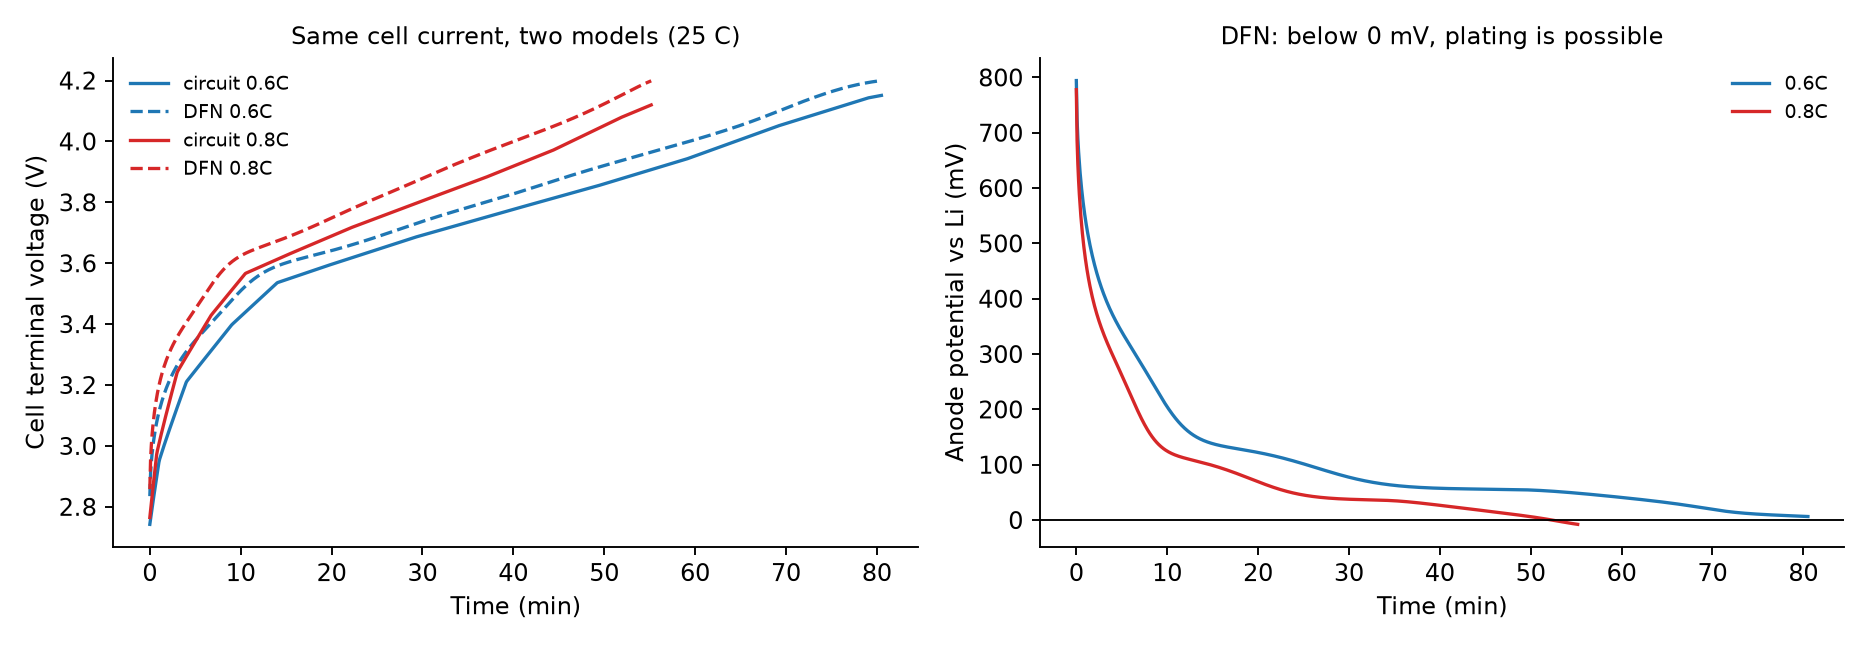
\includegraphics[width=\textwidth]{fig_echem_replay.png}
\caption{Left: terminal voltage of the circuit and of the DFN for the same cell current. Right: DFN negative-electrode potential.}\label{fig:replay}
\end{figure}
\begin{figure}[H]
\centering
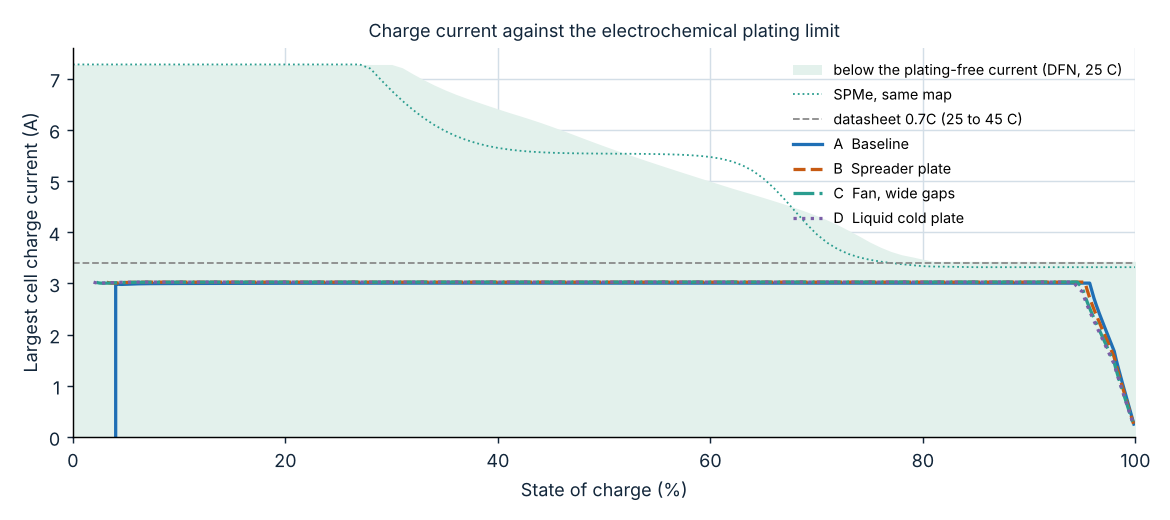
\includegraphics[width=0.92\textwidth]{fig_plating.png}
\caption{Largest cell charge current of the three designs during the first charge (35\,\degC\ ambient, 0.6C) against the plating-free current.}\label{fig:plating}
\end{figure}
Reading. At 0.6C the DFN stays above 0\,mV and the platform ratio is below 100\,\%. At 0.8C the DFN goes below 0\,mV and the platform ratio is above 100\,\%, so the map-based check and the direct DFN replay agree on both cases. The circuit voltage is below the DFN voltage during the CC phase because the Chen2020 cell is about 28\,\% more resistive than the datasheet cell (38 against 30\,m$\Omega$ at 30\,s).

\textbf{Limits of this layer.}
\begin{itemize}
\item The Chen2020 set has no temperature dependence (Section~\ref{sec:val}). The screen is evaluated only for cells at 25\,\degC\ or above, and the charge time spent below 25\,\degC\ is reported (\texttt{plating\_unrated\_s}). Plating risk rises when the cell is colder, so the screen says nothing about cold charging. The datasheet 0.3C limit below 25\,\degC\ stays the controlling rule there.
\item The map is for CC charge from empty. Charging from a partly charged state, or after a rest, changes the concentration gradients.
\item SOC is rated-capacity based in the circuit and accepted-charge based in the map (4.89\,Ah on the map scale). They differ by about 1\,\%.
\item The electrochemical layer does not feed temperature, energy or charge time. Those still come from the circuit and thermal network.
\item The set is a research fit of one M50 cell, not an LG model.
\end{itemize}


%--------------------------------------------------------------------
\section{Liquid cooling: Design D}\label{sec:liquid}
%--------------------------------------------------------------------
\emph{Source: \texttt{liquid\_parts}, \texttt{build\_thermal} and \texttt{simulate} in \texttt{bms/sim.py}; \texttt{Design} and the parts roll-up in \texttt{bms/design.py}; checks LQ1 to LQ4 in \texttt{bms/checks.py}; \texttt{bms/study.py}.}

\textbf{Purpose and status.} Design D asks whether an aluminium cold plate with a water-glycol loop and a small radiator controls cell temperature better than designs A, B and C. It is added to the same thermal network. Designs A, B and C are untouched: their results are identical to the values in the earlier sections (tested in \texttt{tests/test\_model.py}). Every liquid-loop parameter is an engineering estimate or a placeholder. \textbf{None of it is a measurement or a manufacturer specification, and the model has not been validated against a test.}

\subsection{Nodes and heat paths}
Two nodes are added after the $N$ cell nodes: the cold plate $p$ (temperature $T_p$, heat capacity $C_p=m_pc_{p,\mathrm{Al}}$) and the coolant $c$ (temperature $T_c$, heat capacity $C_c=\rho V c_{p,\mathrm{cool}}$). The paths are
\begin{enumerate}
\item cell $k$ to plate through its thermal pad, $G_{\mathrm{pad}}=k_{\mathrm{pad}}A_{\mathrm{pad}}/t_{\mathrm{pad}}$ (the same expression as the spreader design),
\item plate to coolant, with a heat-exchanger conductance $UA_p$,
\item coolant transport around the loop, $\dot Q=\dot m\,c_{p,\mathrm{cool}}\,(T_{\mathrm{out}}-T_{\mathrm{in}})$,
\item coolant to ambient air through the radiator, with conductance $UA_r$,
\item the cells still lose a little heat to the air from their sides, as in design A.
\end{enumerate}
The coolant capacity rate is $\dot C=\dot m\,c_{p,\mathrm{cool}}$ (W/K). It sets how much of each conductance is actually available at a given flow.

\subsection{Heat-exchanger conductances}
For a fluid stream of capacity rate $\dot C$ exchanging heat with a body held at a fixed temperature through a conductance $UA$, the heat transferred per kelvin of temperature difference is
\begin{equation}
\varepsilon_x=1-\exp\!\Big(-\frac{UA_x}{\dot C}\Big),\qquad G_x=\dot C\,\varepsilon_x,\qquad x\in\{p,\ r\}.
\end{equation}
This is the effectiveness--NTU result for the case where the other side has a much larger capacity rate (the plate and the air stream). It is an initial lumped approximation, not a CFD result. With no flow, $\dot C=0$ and both conductances are zero, so a stopped pump isolates the plate from the coolant. The radiator conductance with its fan stopped is $UA_r$ multiplied by 0.25 (ASSUMPTION).

\subsection{Governing equations}
The radiator returns the coolant to the plate inlet at
\begin{equation}
T_{\mathrm{in}}=T_c-\varepsilon_r\,(T_c-T_{\mathrm{amb}}),\qquad
Q_p=G_p\,(T_p-T_{\mathrm{in}}),\qquad
T_{\mathrm{out}}=T_{\mathrm{in}}+\frac{Q_p}{\dot C},
\end{equation}
so $Q_p=\dot m\,c_{p,\mathrm{cool}}(T_{\mathrm{out}}-T_{\mathrm{in}})$ holds by construction. The two new node equations are
\begin{align}
C_p\frac{dT_p}{dt}&=\sum_{k}G_{\mathrm{pad}}(T_k-T_p)-Q_p-G_{\mathrm{air}}(T_p-T_{\mathrm{amb}}),\\
C_c\frac{dT_c}{dt}&=Q_p-G_r\,(T_c-T_{\mathrm{amb}})+\eta_{\mathrm{pump}}P_{\mathrm{pump}} .
\end{align}
The cell equations are those of Section~\ref{sec:therm} with one extra term, $-G_{\mathrm{pad}}(T_k-T_p)$. The pump heat enters the coolant at the radiator inlet with $\eta_{\mathrm{pump}}=1$ (ASSUMPTION: all electrical power ends as heat in the fluid). The radiator fan power is not added as heat because it heats the air stream. In matrix form the network is $C\,\dot T=-KT+w\,T_{\mathrm{amb}}+q$ as before, with $K$ not symmetric because heat is carried by the flow. The same backward Euler step and the same precomputed inverse are used. A second inverse, with the pump stopped, is used during rest phases (when the controller stops the pump and radiator fan) and after a pump fault.

\textbf{Steady state.} Setting the derivatives to zero and eliminating $T_{\mathrm{in}}$ gives a series conductance between the plate and ambient for heat from the cells,
\begin{equation}
G_{\mathrm{eff}}=\dot C\,\frac{\varepsilon_r\varepsilon_p}{\varepsilon_r+\varepsilon_p-\varepsilon_r\varepsilon_p}\ \longrightarrow\ \frac{UA_rUA_p}{UA_r+UA_p}\quad(\dot C\to\infty).
\end{equation}
With the default values $\dot C=100.5$\,W/K, $\varepsilon_r=0.077$, $\varepsilon_p=0.058$, so $G_{\mathrm{eff}}=3.43$\,W/K against $3.43$\,W/K at infinite flow. Cells cannot be cooled below ambient: $T_c\ge T_{\mathrm{amb}}$ in every case, which the tests check. The plate-to-ambient temperature rise for about 9\,W of heat is therefore roughly 2.6\,K, and the pad and spread add the rest.

\subsection{Auxiliary energy, heat and net usable energy}
Pump and radiator fan power are electrical loads. The auxiliary energy of a run is $E_{\mathrm{aux}}=\int(P_{\mathrm{pump}}+P_{\mathrm{fan,rad}})\,dt$, and the net usable energy of the first discharge is
\begin{equation}
E_{\mathrm{use}}=E_{\mathrm{dis}}-\int_{\mathrm{discharge}}(P_{\mathrm{pump}}+P_{\mathrm{fan,rad}})\,dt ,
\end{equation}
the same rule as the fan of design C. Check I4 compares pump and fan power with module power. The pump heat enters the thermal network and its electrical energy enters $E_{\mathrm{aux}}$; these are two views of one energy and are not counted twice in either place.

\textbf{Energy conservation.} Heat made in the cells and interconnects plus pump heat equals the heat stored in cells, plate and coolant plus the heat sent to ambient (air convection and radiator). For the default two-cycle run this closes to 0.006\,Wh out of 49.3\,Wh, and the coolant node balances at every step to $10^{-11}$\,W away from the steps where the pump switches (\texttt{tests/test\_model.py}).

\subsection{Checks added for the liquid loop}
\begin{longtable}{@{}p{0.9cm}p{5.2cm}p{3.1cm}p{5.7cm}@{}}
\toprule
ID & Quantity & Pass condition & Basis \\
\midrule
\endhead
LQ1 & coolant rise across the plate, $T_{\mathrm{out}}-T_{\mathrm{in}}$ & $\le 5$\,K & flow adequacy, design guideline \\
LQ2 & $G_r(T_{\mathrm{req}}-T_{\mathrm{amb}})$ against the mean heat load (cells, bus, pump) & $\ge 100$\,\% & the radiator can hold the coolant at the requirement; zero at $T_{\mathrm{amb}}\ge T_{\mathrm{req}}$ \\
LQ3 & hottest cell minus coolant & $\le 10$\,K & share used by pad, plate and plate-to-coolant resistance \\
LQ4 & pad is an electrical insulator & yes & design rule, cannot be simulated; cell cans sit at different potentials \\
\bottomrule
\end{longtable}
The 5\,K and 10\,K limits are guidelines, not datasheet values. The ranking counts liquid-loop fails after requirement fails.

\subsection{Parameters and sources}
\begin{table}[H]
\centering\scriptsize
\begin{tabular}{@{}p{5.4cm}p{1.4cm}p{1.5cm}p{6.7cm}@{}}
\toprule
Parameter & Value & Unit & Source \\
\midrule
Coolant type & Water-glycol 50/50 & - & preset names a typical mixture \\
Coolant specific heat & 3350 & J/kg/K & ESTIMATE: typical handbook value near 30 to 40 C, not a supplier specification \\
Coolant density & 1065 & kg/m3 & ESTIMATE: typical handbook value, not a supplier specification \\
Coolant volume in the whole loop & 0.35 & L & ESTIMATE: plate channels, hoses, radiator, reservoir \\
Coolant mass flow rate & 0.03 & kg/s & ESTIMATE: small DC pump class, oversized for about 9 W of heat \\
Coolant temperature at the start & ambient & C & input: clipped to ambient or above (no refrigeration) \\
Cold plate area & 80 & cm2 & ESTIMATE: 4S3P footprint is about 61 cm2 \\
Cold plate thickness & 6 & mm & ESTIMATE: milled channels inside \\
Cold plate mass & 0.085 & kg & ESTIMATE: area x thickness x 2700 kg/m3 x 65 \% solid fraction \\
Cold plate to coolant conductance UA & 6 & W/K & ESTIMATE: laminar channel, h about 400 W/m2/K x 0.015 m2 wetted \\
Radiator UA, fan on & 8 & W/K & ESTIMATE: compact radiator with an 80 to 92 mm fan, no supplier data \\
Pump electrical power & 4 & W & ESTIMATE: small brushless DC pump class \\
Radiator fan electrical power & 2 & W & ESTIMATE: 80 to 92 mm fan class \\
Thermal pad conductivity & 1.5 & W/m/K & ASSUMPTION: shared with the spreader design \\
Thermal pad thickness & 1 & mm & ASSUMPTION \\
Pad contact area per cell & 3.5 & cm2 & cell base area, 21.1 mm diameter (DS 3.2) \\
Pump, radiator, fan, hoses, fittings: mass & 250 & g & PLACEHOLDER: weigh the real parts \\
Same parts: packaged volume & 250 & cm3 & PLACEHOLDER \\
Loop hardware cost & 1650 & INR & PLACEHOLDER, not a quote. Replace with supplier prices \\
Radiator UA without its fan, share of the fan-on value & 0.25 & - & ASSUMPTION: sim.RAD\_NATURAL\_FRACTION \\
Pump heat entering the coolant, share of pump power & 1.0 & - & ASSUMPTION: wet-rotor pump, sim.PUMP\_HEAT\_FRACTION \\
\bottomrule
\end{tabular}
\caption{Design D parameters. ESTIMATE and PLACEHOLDER values are not measurements or supplier specifications.}
\end{table}

\subsection{Result: four cooling systems, default case}
35\,\degC\ ambient, 1C discharge, 0.6C charge, two cycles.
\begin{table}[H]
\centering\scriptsize
\begin{tabular}{@{}p{4.1cm}cccc@{}}
\toprule
 & A & B & C & D \\
\midrule
Peak cell temperature (\degC) & 57.3 & 47.7 & 41.8 & 38.8 \\
Average cell temperature (\degC) & 44.8 & 42.1 & 38.5 & 37.3 \\
Cell-to-cell spread (K) & 4.67 & 0.21 & 0.82 & 0.12 \\
Net usable energy (Wh) & 202.3 & 203.6 & 203.9 & 198.9 \\
Charge time (min) & 136 & 104 & 105 & 106 \\
Round-trip efficiency (\%) & 94.6 & 94.5 & 94.2 & 94.0 \\
Auxiliary energy, whole run (Wh) & 0.0 & 0.0 & 4.9 & 32.9 \\
\quad pump (Wh) & 0.0 & 0.0 & 0.0 & 21.9 \\
\quad radiator fan (Wh) & 0.0 & 0.0 & 0.0 & 11.0 \\
\quad module fan (Wh) & 0.0 & 0.0 & 4.9 & 0.0 \\
Mass (g) & 878 & 952 & 890 & 1592 \\
Estimated cost (INR, placeholders) & 6226 & 6586 & 6376 & 8116 \\
Volume (cm$^3$) & 430 & 467 & 550 & 728 \\
Energy density (Wh/kg) & 230 & 214 & 229 & 125 \\
Energy density (Wh/L) & 470 & 436 & 371 & 273 \\
\midrule
Fails: datasheet, requirement, interface, liquid-loop & 1, 2, 2, 0 & 0, 1, 1, 0 & 0, 0, 0, 0 & 0, 3, 1, 0 \\
Weighted score (four designs) & 0.500 & 0.789 & 0.890 & 0.440 \\
\bottomrule
\end{tabular}
\caption{Comparison of the four cooling systems. Score is the min--max weighted score over the four designs.}\label{tab:cmp4}
\end{table}
Reading. Design D has the lowest and most uniform temperatures (38.8\,\degC\ peak against 41.8 for C, spread 0.12\,K), but it is the heaviest, largest and most expensive design (1592\,g, 728\,cm$^3$, INR 8116, all from placeholder part values) and it spends 32.9\,Wh on pump and fans over the two-cycle run, which lowers net usable energy by 5.9\,Wh in the first discharge. It fails the mass, cost and volume requirements and the fan-and-pump share check, so it ranks 3 of 4 and the ranking recommends C  Fan, wide gaps. Design C already meets the 45\,\degC\ requirement at this operating point, so the extra 3\,K of margin does not pay for itself here. With the requirement limits of mass, volume and cost relaxed, D would rank second behind C in this case; the ranking is a result of the simulation and of the editable limits, not a built-in preference.

\begin{figure}[H]
\centering
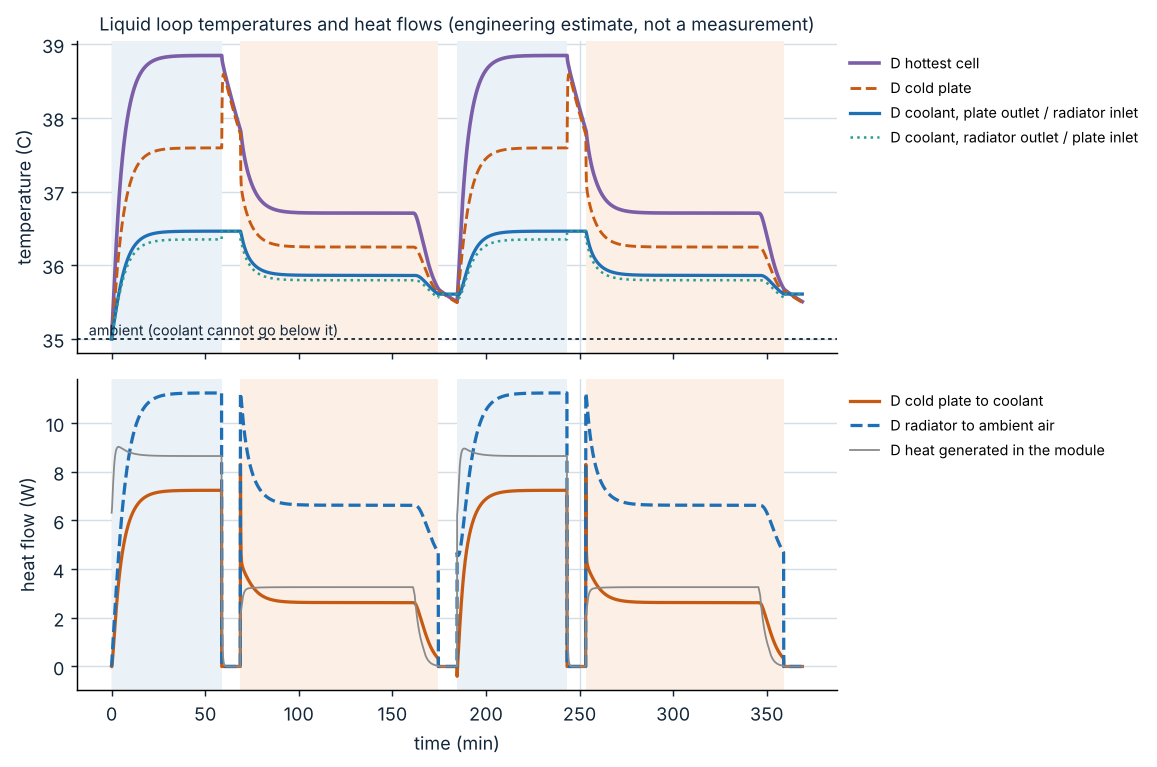
\includegraphics[width=0.95\textwidth]{fig_coolant.png}
\caption{Design D: hottest cell, plate and coolant temperatures, and heat flows. The coolant cannot fall below ambient.}
\end{figure}
\begin{figure}[H]
\centering
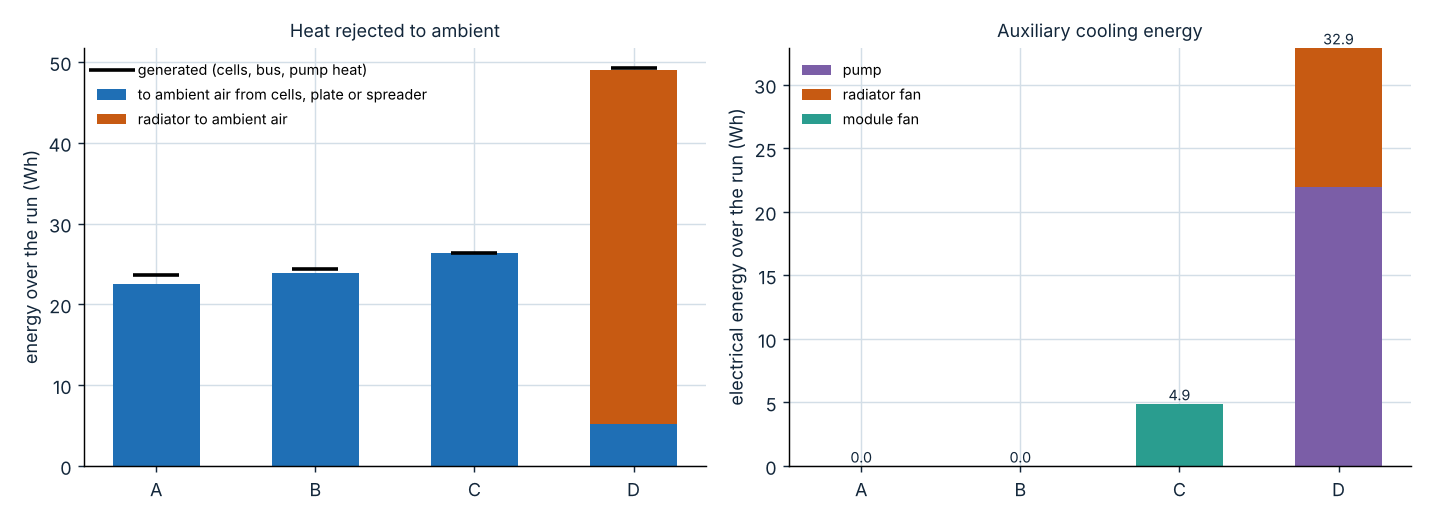
\includegraphics[width=\textwidth]{fig_heat_removal.png}
\caption{Where the heat goes (left) and what the cooling hardware costs in electrical energy (right), whole two-cycle run.}
\end{figure}

\subsection{Ambient temperature, discharge rate and repeated cycles}
Three cycles, 0.6C charge (limited to the discharge rate when that is lower). Peak cell temperature in \degC; the text below gives the highest ambient at which the radiator can hold the coolant at the 45\,\degC\ requirement with the mean heat load of each case.
\begin{table}[H]
\centering\scriptsize
\begin{tabular}{@{}cc cccc@{}}
\toprule
Ambient (\degC) & Discharge & A & B & C & D \\
\midrule
25 & 0.5C & 34.0 & 29.7 & 27.3 & 26.5 \\
25 & 1C & 48.9 & 39.7 & 33.2 & 29.6 \\
25 & 1.5C & 65.7 & 51.0 & 40.6 & 34.0 \\
35 & 0.5C & 42.5 & 38.9 & 36.9 & 36.3 \\
35 & 1C & 57.4 & 47.7 & 41.8 & 38.8 \\
35 & 1.5C & 66.1 & 60.0 & 48.9 & 42.5 \\
45 & 0.5C & 51.5 & 48.4 & 46.6 & 46.2 \\
45 & 1C & 62.8 & 57.4 & 51.3 & 48.4 \\
45 & 1.5C & 63.6 & 60.3 & 58.8 & 52.1 \\
\bottomrule
\end{tabular}
\caption{Peak cell temperature over three cycles (\degC). Values above 45 are outside the requirement.}\label{tab:study}
\end{table}
Within the 45\,\degC\ requirement: A 2, B 3, C 5, D 6 of 9 cases. At 25\,\degC\ and 35\,\degC\ ambient D is the coolest design at every rate, by 0.6 to 6.6\,K below C. At 45\,\degC\ ambient no design stays within the requirement and none completes a charge: the BMS charge trip does not release until the cells fall below 40\,\degC, and the radiator cannot take the coolant below ambient. The radiator can hold the coolant at the requirement temperature only up to an ambient of 43.4 to 44.5\,\degC\ (mean heat load of each case), so liquid cooling with a radiator to ambient air does not remove the need for a cooler environment or a chiller above that. The peak of the last cycle never exceeds the peak of the first cycle by more than 0.2\,K for D (no accumulation) in the cases below 45\,\degC.

\subsection{Fault cases}
Design D, 35\,\degC, 1C, the BMS temperature trips unchanged.
\begin{table}[H]
\centering\scriptsize
\begin{tabular}{@{}p{3.3cm}cccp{4.6cm}@{}}
\toprule
Fault & Peak (\degC) & Mean (\degC) & Min above 45 & Result \\
\midrule
Healthy loop & 38.8 & 37.3 & 0 & within the requirement \\
Flow reduced to 50 \% & 38.8 & 37.3 & 0 & within the requirement \\
Flow reduced to 25 \% & 38.8 & 37.3 & 0 & within the requirement \\
Radiator fan failed & 41.7 & 39.3 & 0 & within the requirement \\
Pump stops at 10 min & 51.6 & 43.0 & 105 & above the 45 C charge limit, BMS blocks charging \\
No flow from the start & 51.6 & 43.2 & 111 & above the 45 C charge limit, BMS blocks charging \\
\bottomrule
\end{tabular}
\caption{Coolant-side faults for design D.}
\end{table}
Cutting the flow to 25\,\% changes the peak by less than 0.1\,K, because the design flow is much larger than needed. A radiator-fan failure raises the peak to 41.7\,\degC. A pump failure is the dangerous case: after the pump stops at 10 minutes the peak reaches 51.6\,\degC, above the 45\,\degC\ charge limit, and the BMS blocks charging for about 58\,min. The BMS sees only cell temperature, so it detects the fault late.

\subsection{Safety and engineering risks outside the model}
\begin{itemize}
\item \textbf{Electrical isolation.} The cans of 21700 cells sit at the potential of their series group, up to 16.8\,V across the module. The pad must be a dielectric with a rated breakdown voltage, and the check LQ4 only records the design rule. An insulation-resistance test is needed.
\item \textbf{Coolant leakage.} Water-glycol is conductive. A leak at the cells or busbars is a short-circuit and corrosion risk. Not modelled; use a sealed plate, keep fittings off the electrical side, add leak detection and pressure-test the loop.
\item \textbf{Flow and pump failure.} The fault cases show the temperature consequence. The BMS has no flow sensor, so a pump fault is caught late, by the temperature trips.
\item \textbf{Thermal interface resistance.} It is lumped in the pad conductivity and thickness. Contact pressure and ageing are not modelled.
\item \textbf{Over-temperature protection.} The 45\,\degC\ charge and 60\,\degC\ discharge trips act on the sensor cell. In design D the spread is below 0.2\,K, so the corner sensor reads the module well.
\item Pressure drop, flow distribution, air locks, fouling, freezing and boiling are not modelled.
\end{itemize}

\subsection{Limits of the liquid model}
\begin{itemize}
\item Two thermal nodes for the loop and effectiveness conductances: no flow network, no pressure drop, no transport delay. The default time constant of the coolant node ($C_c/G_r\approx 162$\,s) is short against the 58\,min discharge, so a delay would not change the peak much, but it is not tested.
\item All parameters in the table above are estimates or placeholders. Mass, volume and cost of the loop hardware are stand-ins, not quotes. The result that D is heavy and expensive follows from those placeholders and has to be re-run with real parts.
\item The loop has no refrigeration. At or above the 45\,\degC\ requirement it cannot cool the cells to the requirement.
\item The flow is oversized for about 9\,W of heat (coolant rise 0.08\,K). The peak barely moves from 30 down to 3\,g/s, and rises only below about 1\,g/s. A smaller pump is a possible saving that this model does not cost.
\end{itemize}

%--------------------------------------------------------------------
\section{Ranking and recommendation}\label{sec:rank}
%--------------------------------------------------------------------
\emph{Source: \texttt{rank} in \texttt{bms/checks.py}.} For each indicator $j$ with weight $w_j$ and value $x_{j,d}$ for design $d$, the value is min--max normalised across the designs:
\begin{equation}
\hat x_{j,d}=\frac{x_{j,d}-\min_d x_{j,d}}{\max_d x_{j,d}-\min_d x_{j,d}},\qquad
u_{j,d}=\begin{cases}\hat x_{j,d}&\text{higher is better (usable energy)}\\1-\hat x_{j,d}&\text{lower is better (all others)}\end{cases}
\end{equation}
\begin{equation}
S_d=\sum_j w_j\,u_{j,d},\qquad \sum_j w_j=1 .
\end{equation}
If all designs have the same value for an indicator, its contribution is 0 for all. Designs are then ordered by (1) number of datasheet fails, (2) number of electrochemical fails, (3) number of requirement fails, (4) number of liquid-loop fails, (5) score $S_d$ in descending order. A design is \emph{acceptable} if it has no datasheet, electrochemical, requirement or liquid-loop fail. The ranking is computed from the simulated results of every design in the comparison, so it does not assume liquid cooling wins or loses. The first row is the recommendation. Default weights: temperature 0.30, energy 0.15, charge time 0.15, mass 0.15, cost 0.15, volume 0.10. The sidebar sliders are rescaled to sum to 1.

\begin{table}[H]
\centering
\begin{tabular}{@{}lcccc@{}}
\toprule
Indicator & Weight & $u$ (A) & $u$ (B) & $u$ (C) \\
\midrule
Peak temperature & 0.30 & 0.000 & 0.618 & 1.000 \\
Usable energy & 0.15 & 0.000 & 0.793 & 1.000 \\
Charge time & 0.15 & 0.000 & 1.000 & 0.952 \\
Mass & 0.15 & 1.000 & 0.000 & 0.837 \\
Cost & 0.15 & 1.000 & 0.000 & 0.584 \\
Volume & 0.10 & 1.000 & 0.688 & 0.000 \\
\midrule
Weighted score & 1.00 & 0.400 & 0.523 & 0.806 \\
\bottomrule
\end{tabular}
\caption{Worked ranking example. Design C scores highest (0.806) and has no datasheet or requirement fail, so it is the recommendation. Design A scores lowest (0.400) and also has a datasheet fail, so it is ranked last by every criterion.}
\end{table}

%--------------------------------------------------------------------
\section{Graphs and tables: what is plotted}\label{sec:graphs}
%--------------------------------------------------------------------
\emph{Source: \texttt{bms/plots.py}, \texttt{run\_report.py}, \texttt{app.py}.}

\subsection{Hottest cell temperature over the duty cycle}
Plotted: $x=t/60$ in minutes, $y=T_{\max}(t)$ for each design. Blue shading marks discharge phases and orange marks charge phases (taken from the first design, since all designs run the same schedule). The dashed line is the 45\,\degC\ requirement, which is also the datasheet charge limit, so one line carries both labels. The legend value is $T_{\mathrm{peak}}$. In design A the curve flattens near 45\,\degC\ during charge: the corner sensor holds the BMS at its trip level while the hottest cell sits several kelvin above.
\begin{figure}[!htbp]
\centering
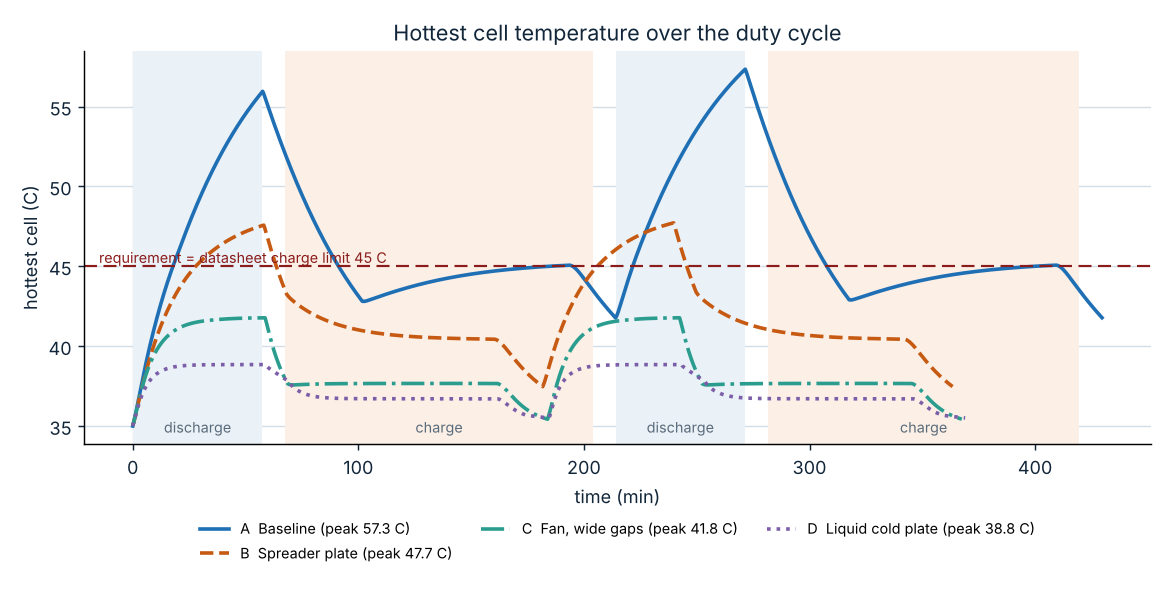
\includegraphics[width=0.92\textwidth]{fig_temperature.png}
\caption{Hottest cell temperature, default scenario.}
\end{figure}

\subsection{Indicators against requirements}
Six bar panels: $T_{\mathrm{peak}}$, $E_{\mathrm{use}}$, $t_{\mathrm{chg}}$, mass, cost and volume. The dashed line in each panel is the requirement from Section~\ref{sec:checks}. In the temperature panel the vertical axis starts at $\min(\text{values},\text{limit})-8$ so that differences are visible.
\begin{figure}[!htbp]
\centering
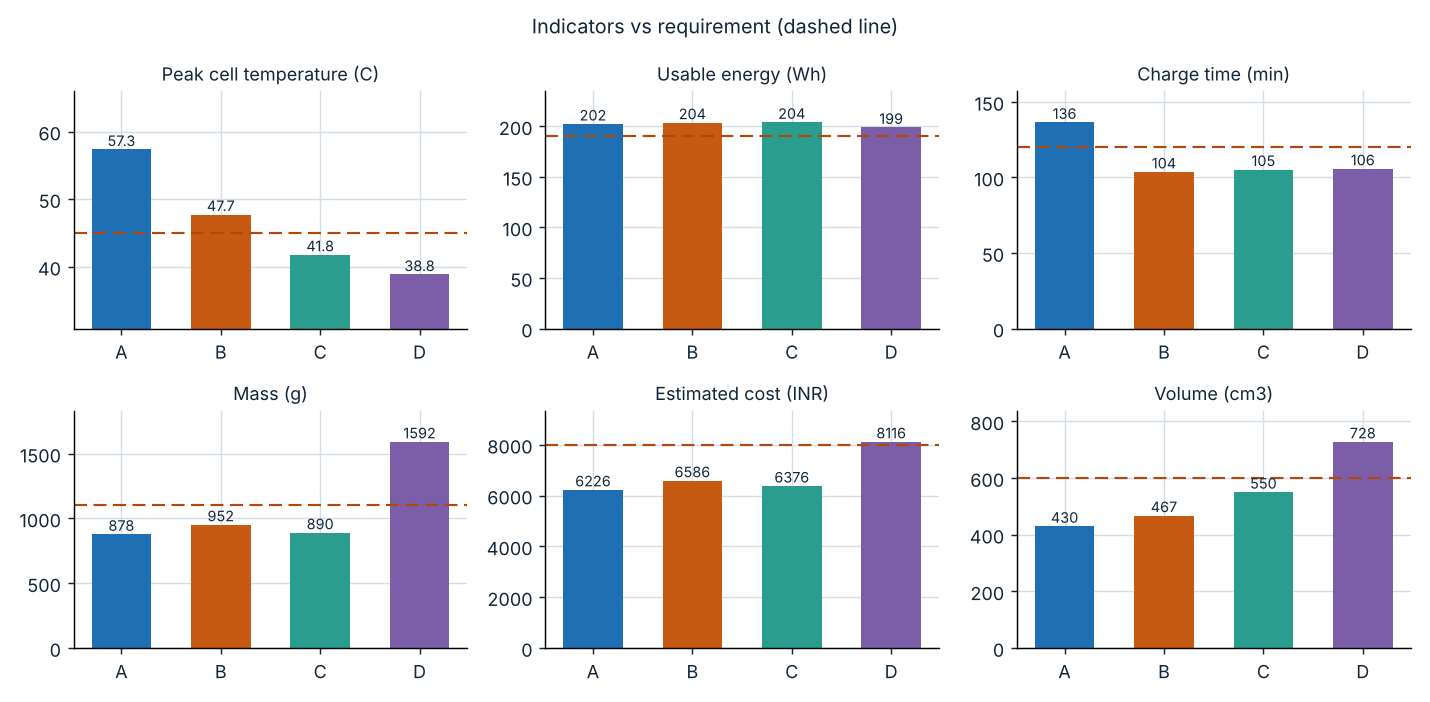
\includegraphics[width=\textwidth]{fig_indicators.png}
\caption{Indicators against requirements.}
\end{figure}

\subsection{Cell temperature map}
For each design, $t^\ast=\arg\max_t T_{\max}(t)$. The map shows the grid $G[i,g]=T_{(g-1)\nP+i}(t^\ast)$ with series groups S1 to S4 as columns and parallel positions P1 to P3 as rows. All maps share one colour scale from the lowest to the highest cell temperature over all designs and all times, so colours compare across designs. In A the interior cells (S2 and S3, row P2) are the hottest. In B and C the plate or the airflow evens out the temperature.
\begin{figure}[!htbp]
\centering
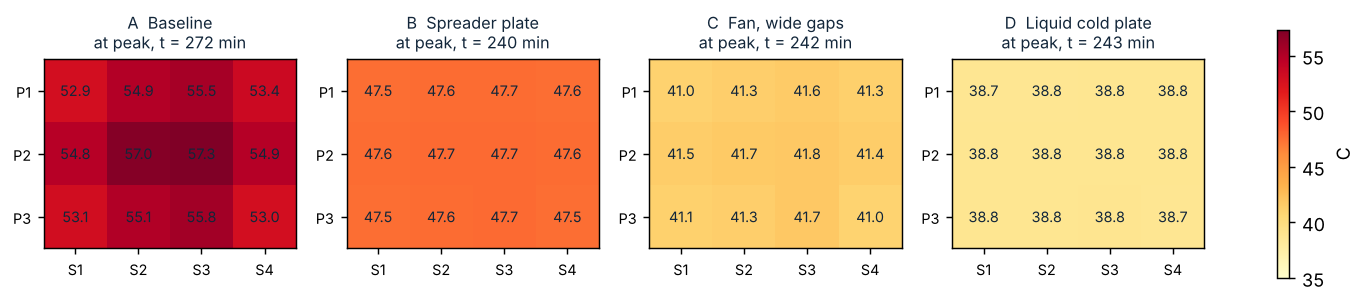
\includegraphics[width=0.95\textwidth]{fig_cell_map.png}
\caption{Cell temperature at the moment of the peak.}
\end{figure}

\subsection{Electrical behaviour}
Three panels against time: $V_{\mathrm{mod}}$, $I$ (positive for discharge, negative for charge), and SOC as $100\,s$. The voltage steps up when the current reverses because the $IR_0$ drop changes sign, then creeps as $V_1$ relaxes during rest, and the current falls during the CV tail.
\begin{figure}[!htbp]
\centering
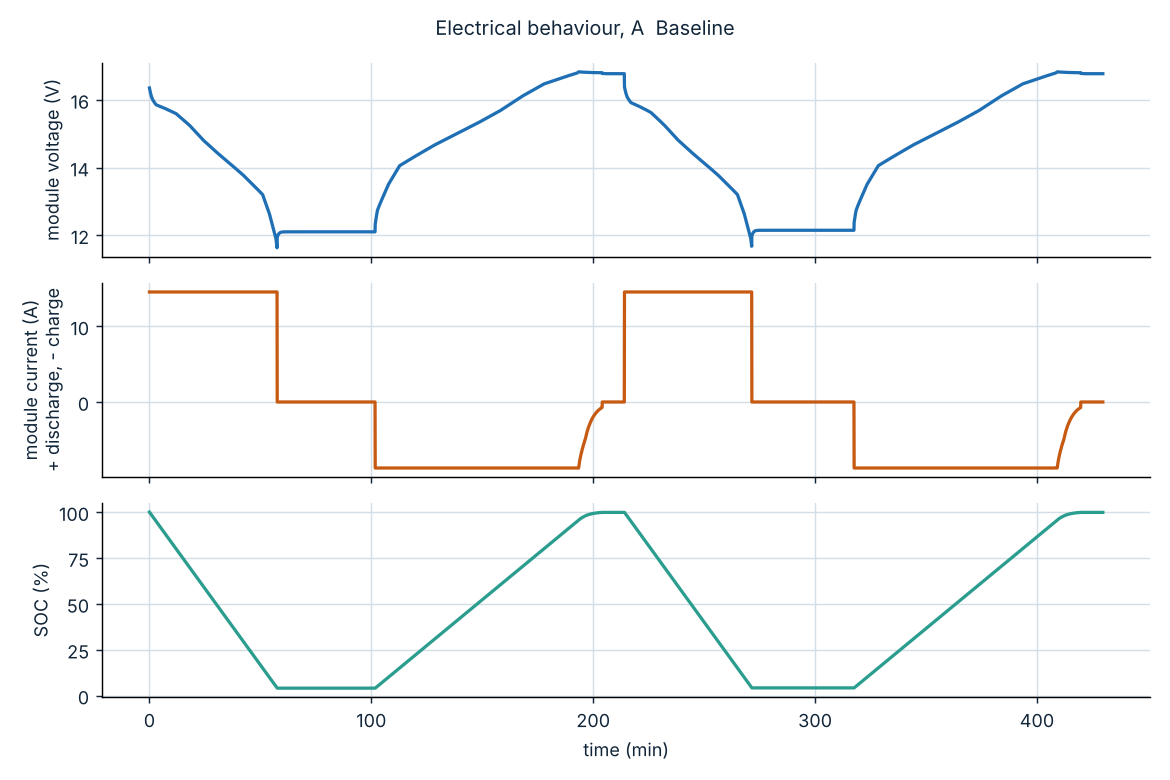
\includegraphics[width=0.85\textwidth]{fig_electrical_baseline.png}
\caption{Voltage, current and SOC for design A.}
\end{figure}

\subsection{Sweeps}
For each value $x$ the model runs one discharge and charge cycle ($\Delta t=10$\,s) and records $T_{\mathrm{peak}}$. In the discharge-rate sweep $c_{\mathrm{dis}}=x$ and $c_{\mathrm{chg}}=\min(x,0.6)$, from 0.5C to 1.5C, the datasheet discharge maximum. In the ambient sweep $T_{\mathrm{amb}}=x$ from 15 to 45\,\degC. The largest rate that stays at or below 45\,\degC\ on a 0.05C grid, one cycle, 35\,\degC\ ambient, is 0.55C for A, 0.85C for B and 1.25C for C.
\begin{figure}[!htbp]
\centering
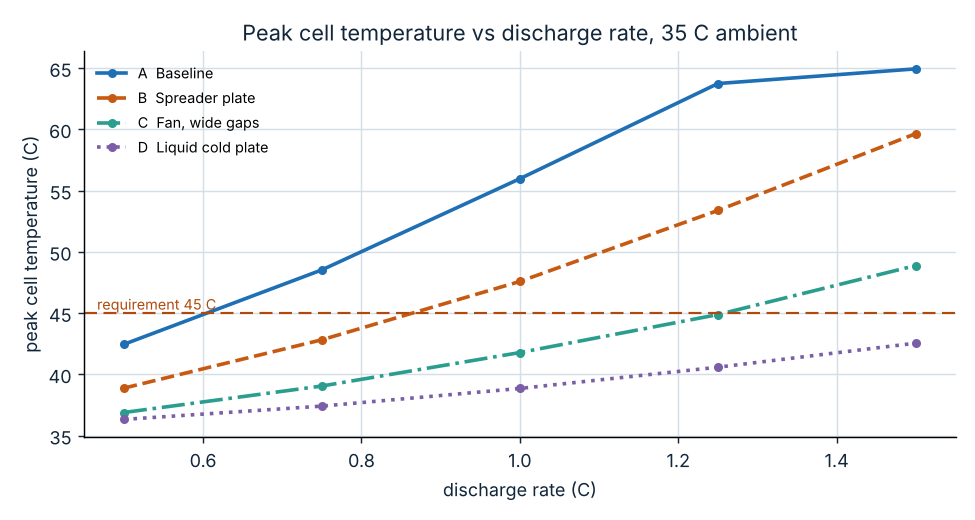
\includegraphics[width=0.75\textwidth]{fig_sweep_crate.png}
\caption{Peak cell temperature versus discharge rate.}
\end{figure}

\subsection{Tables in the dashboard}
\begin{itemize}
\item \textbf{Ranking}: Section~\ref{sec:rank}.
\item \textbf{Indicators}: Section~\ref{sec:ind}, round-trip efficiency shown in \%.
\item \textbf{Checks}: Section~\ref{sec:checks}, with value, limit, unit and reason.
\item \textbf{Traceability}: one row per requirement with component, assumption, model, result (value against limit, PASS or FAIL) and the validation or source. Downloadable as CSV.
\item \textbf{Sensitivity}: Section~\ref{sec:sens}.
\end{itemize}

%--------------------------------------------------------------------
\section{Validation}\label{sec:val}
%--------------------------------------------------------------------
\emph{Source: \texttt{bms/validate.py}, \texttt{tools/pybamm\_crosscheck.py}.} All tests are isothermal, with one ideal cell (no spread, no heating). Because the specification has no rate or charge-time data, each row is labelled \emph{independent} (the model was not set to match it) or \emph{input reproduced} (it only confirms that an input was entered correctly).

\subsection{Against the datasheet and the chart points}
\begin{table}[H]
\centering\scriptsize
\begin{tabular}{@{}p{3.0cm}p{2.0cm}p{2.5cm}p{1.5cm}p{1.8cm}p{4.0cm}@{}}
\toprule
Test & Condition & Datasheet or chart & Model & Diff. & Note \\
\midrule
Energy at 0.2C, 25 C & 0.97 A to 2.5 V & 17.6 Wh min, 18.2 Wh nominal & 17.8 Wh & -0.4 Wh vs nominal & independent: OCV from the electrochemical model, R from DS \\
Mean discharge voltage at 0.2C & 0.97 A to 2.5 V & 3.63 V & 3.68 V & +0.05 V & independent \\
DC resistance, 0.5C pulse & 30 s, 25 C, 50 \% SOC & 30 +/- 6 mOhm & 31.4 mOhm & +1.4 mOhm & input reproduced, not independent \\
DC resistance, 0.5C pulse & 0.5 s, 25 C, 50 \% SOC & 21 to 25 mOhm (3 cells) & 24.9 mOhm & top of range & independent: R0 is fitted to the electrochemical model, not to these points \\
Resistance ratio to 25 C & 10 C & 2.96 (chart means) & 2.96 & +0.00 & input reproduced, not independent. Chart read by eye \\
Resistance ratio to 25 C & 45 C & 0.61 (chart means) & 0.61 & +0.00 & input reproduced, not independent. Chart read by eye \\
Energy vs 25 C, resistance only & 0 C, 0.2C & 80 \% & 94 \% & +14 points & independent: resistance alone does not explain the loss, so the datasheet table is added \\
Energy vs 25 C, with DS table & 0 C, 0.2C & 80 \% & 79 \% & -1 points & input reproduced, not independent \\
Energy vs 25 C, resistance only & -10 C, 0.2C & 70 \% & 86 \% & +16 points & independent: resistance alone does not explain the loss, so the datasheet table is added \\
Energy vs 25 C, with DS table & -10 C, 0.2C & 70 \% & 65 \% & -5 points & input reproduced, not independent \\
Energy vs 25 C, resistance only & 60 C, 0.2C & 95 \% & 100 \% & +5 points & independent: resistance alone does not explain the loss, so the datasheet table is added \\
Energy vs 25 C, with DS table & 60 C, 0.2C & 95 \% & 97 \% & +2 points & input reproduced, not independent \\
\bottomrule
\end{tabular}
\caption{Model against datasheet (DS) and chart (BD).}
\end{table}
Reading. The OCV curve and $R_0+R_1$ reproduce the datasheet energy at 0.2C: 17.8\,Wh against 17.6 minimum and 18.2 nominal, with a mean voltage 0.05\,V above the nominal 3.63\,V. The 0.5\,s resistance of 24.9\,m$\Omega$ is at the top of the 21 to 25\,m$\Omega$ points on the BD chart and was not fitted. Resistance alone predicts 94\,\% energy at 0\,\degC\ and 86\,\% at $-10$\,\degC\ against 80 and 70\,\% in the datasheet, which is why the datasheet table is added for temperature; those rows then match by construction. At 60\,\degC\ the datasheet loses 5\,\% and the resistance model loses none.

\subsection{Against the electrochemical model}
The PB set is run in the DFN model at 25\,\degC\ by \texttt{tools/pybamm\_crosscheck.py}. The set has no temperature dependence (activation energies and entropic coefficients are zero), so it cannot check cold or hot behaviour. Charge times are compared in units of C-hours (time multiplied by the C-rate) so that the 5.12\,Ah DFN cell and the 4.85\,Ah rated cell are on one basis. The last column of the table runs the circuit with the DFN's own resistance, which separates model structure from the resistance difference.
\begin{table}[H]
\centering\scriptsize
\begin{tabular}{@{}p{2.9cm}p{1.9cm}p{1.6cm}p{1.6cm}p{1.2cm}p{2.0cm}p{2.9cm}@{}}
\toprule
Test & Condition & DFN & Circuit & Diff. & Circuit, DFN $R$ & Type \\
\midrule
DC resistance, 0.5C, 30 s, 50 \% SOC & 25 C & 38.4 mOhm & 31.4 mOhm & -7.0 mOhm & - & DFN is above the datasheet 30 +/- 6 mOhm; circuit is set to the datasheet \\
DC resistance, 0.5C, 0.5 s, 50 \% SOC & 25 C & 27.1 mOhm & 24.9 mOhm & -2.2 mOhm & - & measured cells: 21 to 25 mOhm (BD chart) \\
Capacity vs 0.2C & 0.2C, 25 C & 100.0 \% & 100.0 \% & +0.0 & 100.0 \% & independent \\
Energy vs 0.2C & 0.2C, 25 C & 100.0 \% & 100.0 \% & +0.0 & 100.0 \% & independent \\
Capacity vs 0.2C & 0.5C, 25 C & 99.1 \% & 99.7 \% & +0.6 & 99.6 \% & independent \\
Energy vs 0.2C & 0.5C, 25 C & 97.2 \% & 98.3 \% & +1.1 & 97.9 \% & independent \\
Capacity vs 0.2C & 1.0C, 25 C & 97.5 \% & 99.2 \% & +1.7 & 99.0 \% & independent \\
Energy vs 0.2C & 1.0C, 25 C & 93.1 \% & 95.4 \% & +2.4 & 94.4 \% & independent \\
Capacity vs 0.2C & 1.5C, 25 C & 95.8 \% & 98.7 \% & +2.9 & 98.3 \% & independent \\
Energy vs 0.2C & 1.5C, 25 C & 88.9 \% & 92.6 \% & +3.7 & 90.9 \% & independent \\
Charge time to end current, in C-hours & 0.3C CC-CV, 25 C & 1.221 h x C & 1.056 h x C & -14 \% & 1.075 h x C (-12 \%) & independent, 50 mA end current \\
Charge time to end current, in C-hours & 0.5C CC-CV, 25 C & 1.200 h x C & 1.076 h x C & -10 \% & 1.101 h x C (-8 \%) & independent \\
Charge time to end current, in C-hours & 0.6C CC-CV, 25 C & 1.277 h x C & 1.110 h x C & -13 \% & 1.149 h x C (-10 \%) & independent \\
Charge time to end current, in C-hours & 0.7C CC-CV, 25 C & 1.364 h x C & 1.150 h x C & -16 \% & 1.204 h x C (-12 \%) & independent, C/20 end current \\
\bottomrule
\end{tabular}
\caption{Equivalent circuit against the PyBaMM DFN model, 25\,\degC.}
\end{table}
Reading. With the datasheet resistance the circuit gives energy within 2.4 points of the DFN at 1C and 3.7 at 1.5C, and these are optimistic because the DFN cell is 28\,\% more resistive (38 against 30\,m$\Omega$). With the DFN's resistance the gap is smaller. Charge time is 10 to 16\,\% shorter than the DFN at 0.3C to 0.7C, so the charge times in this report are lower bounds. A second polarisation branch did not improve the pulse fit, so the remaining difference is not a matter of branch count. A plausible cause is the SOC dependence of diffusion in the DFN, which a fixed linear branch does not follow; this was not tested.

%--------------------------------------------------------------------
\section{Sensitivity to the uncertain inputs}\label{sec:sens}
%--------------------------------------------------------------------
\emph{Source: \texttt{bms/sensitivity.py}.} One input at a time is moved between the two levels shown, with the default scenario and $\Delta t=10$\,s, and the four designs are re-ranked. The last four inputs apply to the liquid loop only, so A, B and C do not move.
\begin{table}[H]
\centering\scriptsize
\begin{tabular}{@{}p{4.6cm}p{1.5cm}cccc>{\centering\arraybackslash}p{1.9cm}@{}}
\toprule
Input & Level & A (\degC) & B (\degC) & C (\degC) & D (\degC) & Order \\
\midrule
Base case & - & 57.4 & 47.7 & 41.8 & 38.8 & C $>$ B $>$ D $>$ A \\
Natural convection h, +/- 30 \% & 7 & 61.1 & 51.6 & 42.5 & 39.0 & C $>$ D $>$ B $>$ A \\
Natural convection h, +/- 30 \% & 13 W/m2K & 54.0 & 45.3 & 41.2 & 38.7 & C $>$ B $>$ D $>$ A \\
Gap exposure length, 2 / 4.5 mm & 2 & 54.3 & 46.8 & 41.1 & 38.8 & C $>$ B $>$ D $>$ A \\
Gap exposure length, 2 / 4.5 mm & 4.5 mm & 60.7 & 48.6 & 43.2 & 38.9 & C $>$ B $>$ D $>$ A \\
Forced convection coefficient, +/- 30 \% & -30 \% & 57.4 & 47.7 & 43.1 & 38.8 & C $>$ B $>$ D $>$ A \\
Forced convection coefficient, +/- 30 \% & +30 \% & 57.4 & 47.7 & 40.8 & 38.8 & C $>$ B $>$ D $>$ A \\
Cell specific heat, 800 / 1100 & 800 & 58.2 & 47.9 & 41.8 & 38.8 & C $>$ B $>$ D $>$ A \\
Cell specific heat, 800 / 1100 & 1100 J/kgK & 55.9 & 47.3 & 41.8 & 38.8 & C $>$ B $>$ D $>$ A \\
Cell resistance, +/- 20 \% (DS tolerance) & -20 \% & 53.6 & 45.6 & 40.7 & 38.3 & C $>$ B $>$ D $>$ A \\
Cell resistance, +/- 20 \% (DS tolerance) & +20 \% & 61.1 & 49.9 & 42.8 & 39.4 & C $>$ B $>$ D $>$ A \\
Resistance spread, 0 / 10 \% & 0 \% & 57.7 & 47.8 & 42.0 & 38.8 & C $>$ B $>$ D $>$ A \\
Resistance spread, 0 / 10 \% & 10 \% & 57.0 & 47.6 & 42.0 & 38.9 & C $>$ B $>$ D $>$ A \\
Ambient temperature, 30 / 40 C & 30 C & 53.0 & 43.5 & 37.5 & 34.2 & C $>$ B $>$ D $>$ A \\
Ambient temperature, 30 / 40 C & 40 C & 60.6 & 52.4 & 46.3 & 43.5 & C $>$ D $>$ B $>$ A \\
Thermal pad conductivity, 1.0 / 2.5 & 1.0 & 57.4 & 47.8 & 41.8 & 39.3 & C $>$ B $>$ D $>$ A \\
Thermal pad conductivity, 1.0 / 2.5 & 2.5 W/mK & 57.4 & 47.6 & 41.8 & 38.4 & C $>$ B $>$ D $>$ A \\
Radiator UA, +/- 30 \% & -30 \% & 57.4 & 47.7 & 41.8 & 39.3 & C $>$ B $>$ D $>$ A \\
Radiator UA, +/- 30 \% & +30 \% & 57.4 & 47.7 & 41.8 & 38.6 & C $>$ B $>$ D $>$ A \\
Plate-to-coolant UA, +/- 30 \% & -30 \% & 57.4 & 47.7 & 41.8 & 39.2 & C $>$ B $>$ D $>$ A \\
Plate-to-coolant UA, +/- 30 \% & +30 \% & 57.4 & 47.7 & 41.8 & 38.6 & C $>$ B $>$ D $>$ A \\
Coolant flow, 50 / 150 \% & 50 \% & 57.4 & 47.7 & 41.8 & 38.8 & C $>$ B $>$ D $>$ A \\
Coolant flow, 50 / 150 \% & 150 \% & 57.4 & 47.7 & 41.8 & 38.9 & C $>$ B $>$ D $>$ A \\
Liquid loop hardware cost, 50 / 200 \% & 50 \% & 57.4 & 47.7 & 41.8 & 38.8 & C $>$ B $>$ D $>$ A \\
Liquid loop hardware cost, 50 / 200 \% & 200 \% & 57.4 & 47.7 & 41.8 & 38.8 & C $>$ B $>$ D $>$ A \\
\bottomrule
\end{tabular}
\caption{Peak cell temperature of each design and the resulting order.}
\end{table}
Design C ranks first in 25 of 25 cases. D ranks second in 2 and third in 23; B ranks second in 23. A is last in every case. D has the lowest peak temperature in all 25 cases, but it stays behind C (and usually B) because it fails the mass, volume and cost requirements, which do not depend on these inputs. Radiator UA and plate-to-coolant UA of $\pm30$\,\% move the peak of D by -0.2 to +0.5\,K and -0.2 to +0.4\,K, and the coolant flow (50 to 150\,\%) by +0.0 to +0.1\,K, so the temperature result of D is not very sensitive to those estimates around the default point; the cost placeholder does not change the order. The absolute temperatures of A move by about $\pm3.5$\,K for the natural convection coefficient and $\pm3.8$\,K for the cell resistance, and those of C by about $\pm4.5$\,K for a 5\,K change of ambient. The 45\,\degC\ requirement is met by C in 24 of 25 cases (not at 40\,\degC\ ambient, 46.3\,\degC), by D in 25 of 25 (highest 43.5\,\degC, at 40\,\degC\ ambient: 43.5), by B in 1 and by A in none.

%--------------------------------------------------------------------
\section{Automated tests}\label{sec:tests}
%--------------------------------------------------------------------
\texttt{tests/test\_model.py} (run with \texttt{python tests/test\_model.py} or \texttt{pytest}) checks: energy balance over a full run (terminal energy equals OCV energy minus heat minus change of stored polarisation energy, within 3\,\%); SOC and voltage bounds; repeatability with a fixed seed and sensitivity to the seed; temperature symmetry without spread; the datasheet anchors ($0.2Q=0.97$\,A, $0.7Q=3.395$\,A, $1.5Q=7.275$\,A, DCIR inside $30\pm6$\,m$\Omega$, 0.2C energy inside 17.6 to 18.4\,Wh); the current-limit functions; monotonic resistance against temperature; charge-time trends; the ranking order; that no charge current flows while a cell is below 0\,\degC; the plating limit falls with SOC, starts at the 1.5C cap and sits between 0.6C and 0.8C at 90\,\% SOC; check E1 passes at 0.6C and fails at 0.8C; and that cells below 25\,\degC\ are left out of the plating ratio and the time is reported instead (14 tests). Design D adds 15 more: A, B and C unchanged against recorded reference values; heat balance and coolant balance; stability of the network with the pump running, weak and stopped; step-size independence; coolant never below ambient; every liquid parameter moves the temperature in the right direction; pump failure and zero flow; BMS trip on a pump failure; auxiliary energy counted in the net energy; checks LQ1 to LQ4 only for design D; the radiator cannot cool below ambient; the ranking follows the simulated results and does not declare D the winner by default; no drift over three cycles (29 tests in total).

%--------------------------------------------------------------------
\section{Assumptions and limitations}\label{sec:lim}
%--------------------------------------------------------------------
\begin{itemize}
\item The M50 specification is a 2016 tentative draft with no OCV, rate, charge-time or thermal data. The OCV curve is from a research parameter set (PB), and the resistance ratios against temperature are read by eye from a chart (BD).
\item Lumped thermal model: one temperature per cell, no gradients inside a cell, no CFD.
\item One polarisation branch fitted at 25\,\degC. Charge time is 10 to 16\,\% shorter than the electrochemical model and energy at 1C is 2 to 3 points higher, so both are optimistic. The branch time constant follows $R_1$ with temperature, which is an assumption.
\item The electrochemical layer is a 25\,\degC\ screen (Section~\ref{sec:echem}). It is not used for cold behaviour, temperature, energy or charge time, and it does not measure plated lithium.
\item Liquid cooling (Section~\ref{sec:liquid}) is a lumped engineering estimate with no measurement behind it: coolant properties, flow, plate and radiator conductances, pump and fan power, pad properties and the hardware mass, volume and cost are all estimates or placeholders.
\item No ageing. The datasheet states 500 cycles to at least 80\,\% of minimum energy under a 0.33C cycle (\ds{4.3.4}), and BD shows life falling quickly above 1C charge. Neither is tracked.
\item Cold and hot energy loss comes from the \ds{4.4.4} table, measured at 0.2C. Resistance below 10\,\degC\ is an extension of the chart slope.
\item Reversible heat is not modelled.
\item The convection coefficients, gap exposure scale $s_0$, forced-air law, cell specific heat and thermal pad properties are engineering estimates and need a bench test. Section~\ref{sec:sens} shows their effect.
\item Heat conduction through nickel strips and cell ends is ignored, so hotspots are slightly pessimistic.
\item Cost and non-cell mass are placeholders. The cell price needs a supplier quote.
\item The requirement values are editable defaults, not figures from the problem statement.
\item Simulation only. It is not a safety certification of a real pack.
\end{itemize}

%--------------------------------------------------------------------
\appendix
\section{Parameter table with sources}
%--------------------------------------------------------------------
\begin{longtable}{@{}p{4.3cm}p{2.7cm}p{1.6cm}p{6.2cm}@{}}
\toprule
Parameter & Value & Unit & Source \\
\midrule
\endhead
Capacity (rated minimum, defines 1C) & 4.85 & Ah & DS 2.1, 2.9 \\
Nominal voltage & 3.63 & V & DS 2.2 \\
Charge voltage & 4.2 & V & DS 2.5 \\
Discharge cut-off & 2.5 & V & DS 2.7 \\
Cell mass & 0.068 & kg & DS 2.10 \\
Diameter (max) & 0.0211 & m & DS 3.2 \\
Height (max) & 0.07015 & m & DS 3.2 \\
Max continuous discharge, 5 to 60 C (1.5C) & 7.275 & A & DS 2.9 \\
Max continuous discharge, -20 to 5 C (0.3C) & 1.455 & A & DS 2.9 \\
Standard charge current (0.3C) & 1.455 & A & DS 2.4 \\
Max charge current, 0 to 25 C (0.3C) & 1.455 & A & DS 2.6 \\
Max charge current, 25 to 50 C (0.7C) & 3.395 & A & DS 2.6 \\
Charge temperature, min & 0 & C & DS 5.1 \\
Charge temperature, max & 45 & C & DS 5.1 \\
Charge release below & 40 & C & ASSUMPTION: not in datasheet, 5 K hysteresis \\
Discharge temperature, min & -20 & C & DS 5.1 \\
Discharge temperature, max & 60 & C & DS 5.1 \\
Discharge release below & 55 & C & ASSUMPTION: not in datasheet, 5 K hysteresis \\
Charge end current, standard charge & 0.05 & A & DS 2.4 \\
Charge end current, faster charge (C/20) & 0.05 & C & DS 4.2.3 \\
Impedance at 1 kHz (max) & 25 & mOhm & DS 4.3.1 \\
DC resistance, 25 C, 50 \% SOC, 30 s (anchor) & 30 & mOhm & DS 4.3.2 (30 +/- 6) \\
Series resistance R0, 25 C & 24.78 & mOhm & FIT to PB, scaled so R0 + R1 (1 - e\^{}(-30/tau)) = 30 \\
Polarisation resistance R1, 25 C & 14.07 & mOhm & FIT to PB, same scaling \\
Polarisation time constant, 25 C & 65 & s & FIT to PB (tools/fit\_polarisation.py) \\
Specific heat & 900 & J/kg/K & ASSUMPTION: typical 800 to 1100, no M50 value in sources \\
Cell price & 450 & INR & ASSUMPTION: placeholder, use a real quote \\
Open-circuit voltage curve & 16 points & V vs SOC & PB: Chen2020 single-particle model at C/50, 25 C (not a datasheet curve) \\
Resistance and tau vs temperature & x2.96 at 10 C, x1 at 25 C, x0.61 at 45 C & - & BD: DCIR chart read by eye (+/- 2 mOhm). Below 10 C extended, above 45 C held \\
Energy retention vs temperature & 70 \% at -10 C, 80 \% at 0 C, 100 \% at 25 C, 95 \% at 60 C & - & DS 4.4.4 (0.2C discharge) \\
\bottomrule
\end{longtable}

\textbf{Design parameters (defaults).}
\begin{longtable}{@{}p{4.7cm}p{3.2cm}p{3.2cm}p{3.2cm}@{}}
\toprule
Parameter & A Baseline & B Spreader & C Fan, wide gaps \\
\midrule
\endhead
Layout & 4S3P & 4S3P & 4S3P \\
Gap between cells & 1.5\,mm & 1.5\,mm & 4.0\,mm \\
Natural convection $h_{\mathrm{nat}}$ & 10 W/m$^2$/K & 10 W/m$^2$/K & 10 W/m$^2$/K \\
Fan air speed / power & none & none & 2\,m/s / 0.8\,W \\
Spreader plate & none & 125 cm$^2$, 2\,mm Al & none \\
Thermal pad & -- & 1.5 W/m/K, 1\,mm, 5 cm$^2$ per cell & -- \\
BMS sensor on & corner cell & corner cell & corner cell \\
Interconnect resistance & 4\,m$\Omega$ & 4\,m$\Omega$ & 4\,m$\Omega$ \\
\bottomrule
\end{longtable}

\textbf{Scenario and requirement defaults.} Ambient 35\,\degC; discharge 1C; charge 0.6C; 2 cycles; rest 10\,min; resistance spread 5\,\%; seed 7. Requirements: $T_{\mathrm{peak}}\le45$\,\degC; $E_{\mathrm{use}}\ge190$\,Wh; $t_{\mathrm{chg}}\le120$\,min; mass $\le1100$\,g; cost $\le$ INR~8000; volume $\le600$\,cm$^3$; load window 10 to 16.8\,V; cell gap $\ge1$\,mm.

%--------------------------------------------------------------------
\section{Where each formula lives in the code}
%--------------------------------------------------------------------
\begin{center}
\begin{tabular}{@{}p{5.6cm}p{9.3cm}@{}}
\toprule
Item & Location \\
\midrule
OCV, $f(T)$, energy retention, limits, termination current & \texttt{bms/cell.py}: \texttt{ocv}, \texttt{r\_temp\_factor}, \texttt{cap\_retention}, \texttt{i\_chg\_limit}, \texttt{i\_dis\_limit}, \texttt{i\_term} \\
Cell data and sources & \texttt{bms/cell.py}: \texttt{Cell}, \texttt{cell\_param\_table} \\
Thermal matrices & \texttt{bms/sim.py}: \texttt{build\_thermal}, \texttt{h\_effective} \\
Cycle loop, protection, heat & \texttt{bms/sim.py}: \texttt{simulate} \\
Liquid loop: conductances, matrix, indicators & \texttt{bms/sim.py}: \texttt{liquid\_parts}, \texttt{build\_thermal}, \texttt{liquid\_indicators} \\
Liquid parameters, mass, cost, volume & \texttt{bms/design.py}: \texttt{Design}, \texttt{LIQUID\_SOURCES}, \texttt{mass\_g}, \texttt{cost\_inr}, \texttt{volume\_cm3} \\
Ambient and rate study, fault cases & \texttt{bms/study.py}: \texttt{ambient\_rate\_study}, \texttt{failure\_modes} \\
Indicators & \texttt{bms/sim.py}: \texttt{indicators} \\
Mass, cost, volume & \texttt{bms/design.py}: \texttt{mass\_g}, \texttt{cost\_inr}, \texttt{volume\_cm3} \\
Checks, traceability, ranking & \texttt{bms/checks.py}: \texttt{run\_checks}, \texttt{traceability}, \texttt{rank} \\
Validation & \texttt{bms/validate.py}: \texttt{validation\_table} \\
Sensitivity & \texttt{bms/sensitivity.py}: \texttt{run} \\
Plating limit and live replay & \texttt{bms/echem.py}: \texttt{plating\_limit\_c}, \texttt{plating\_limit\_a}, \texttt{replay} \\
OCV table, polarisation fit, DFN cross-check, plating map, replay (need PyBaMM) & \texttt{tools/make\_ocv.py}, \texttt{tools/fit\_polarisation.py}, \texttt{tools/pybamm\_crosscheck.py}, \texttt{tools/make\_plating\_map.py}, \texttt{tools/echem\_replay.py} \\
Tests & \texttt{tests/test\_model.py} \\
Figures & \texttt{bms/plots.py} \\
Report and dashboard & \texttt{run\_report.py}, \texttt{app.py} \\
\bottomrule
\end{tabular}
\end{center}

\end{document}
